\chapter{Phonology}
\label{ch:phonology}

This chapter will present charts depicting the phoneme inventory of Ayeri and
describe the various commonly encountered allophones of both consonants and
vowels. Following this, a detailed statistical analysis of the words found in a
number of translated texts from 2008 to 2016 as well as dictionary entries up
to July 2016 will produce insights into Ayeri's phonotactics. Some notes on
stress patterns and intonation will close the chapter.

\section{Phoneme inventory}

\subsection{Consonants}
\label{subsec:consonants}

\index{consonants|(}%
% \begin{sidewaysfigure}[p]
\afterpage{%
\clearpage% Flush earlier floats (otherwise order might not be correct)
\begin{landscape}
\begin{table}[p]\centering
\caption{Consonant inventory (divergent orthography in brackets)}
\begin{tabu} to \linewidth {B[2l] X[c] X[c] X[c] X[c] X[c] X[c] X[c] X[c] X[c]
X[c] X[c] X[c]}
\toprule\tableheaderfont
	%
	& \multicolumn2{c}{Bilabial}
	& \multicolumn2{c}{Labiodental}
	& \multicolumn2{c}{Alveolar}
	& \multicolumn2{c}{Palatal}
	& \multicolumn2{c}{Velar}
	& \multicolumn2{c}{Glottal}
	\\

\midrule

Plosive
	& p & b	% Bilabials
	&   &  	% Labiodentals
	& t & d	% Alveolars
	&   &  	% Palatals
	& k & g	% Velars
	&   &  	% Glottals
	\\

\midrule

Affricate
	&             &            	% Bilabials
	&             &            	% Labiodentals
	& ʧ~\orth{c} & ʤ~\orth{j}	% Alveolars
	&             &            	% Palatals
	&             &            	% Glottals
	\\

\midrule

Nasal
	&   & m          	% Bilabials
	&   &            	% Labiodentals
	&   & n          	% Alveolars
	&   &            	% Palatals
	&   & ŋ~\orth{ng}	% Velars
	&   &            	% Glottals
	\\

\midrule

Fricative
	&   &  	% Bilabials
	&   & v	% Labiodentals
	& s &  	% Alveolars
	&   &  	% Palatals
	&   &  	% Velars
	& h &  	% Glottals
	\\

\midrule

Tap/Flap
	&   &  	% Bilabials
	&   &  	% Labiodentals
	&   & r	% Alveolars
	&   &  	% Palatals
	&   &  	% Velars
	&   &  	% Glottals
	\\

\midrule

Approximant
	&   &           	% Bilabials
	&   &           	% Labiodentals
	&   & l         	% Alveolars
	&   & j~\orth{y}	% Palatals
	&   &           	% Velars
	&   &           	% Glottals
	\\

\bottomrule
\end{tabu}
\label{tab:consonants}
\end{table}
\end{landscape}
\clearpage
}
%\end{sidewaysfigure}

At 17 consonants, Ayeri has a \textquote{moderately small} inventory, according
to \citet{wals1}. \autoref{tab:consonants} shows the full chart of consonant
phonemes.

\index{allophony|(}
Regarding allophony, /tj kj/ and /dj gj/ are usually realized as [ʧ] and [ʤ],
respecitively, except if a homorganic nasal /n/ or /ŋ/ is preceding: for
instance, \rayr{AMkYu}{ankyu} /ˈaŋkju/ `really' is realized as [ˈaŋkju], not as
*[ˈaŋʧu] or *[ˈanʧu]. It is important to note, however, that besides this
synchronic palatalization process leading to [ʧ] and [ʤ] as
\emph{allophones}, there is also a diachronic one in parallel here---or the
diachronic process is still ongoing. For example, there is no way to predict
whether \xayr{kYun}{cuna}{original, initial}, \xayr{pMtY}{panca}{finally,
eventually}, and \xayr{vtY/}{vac-}{like}, or \xayr{dYrnF}{jaran}{pilgrimage},
\xayr{AgY/}{aja-}{play}, and \xayr{nudY/}{nuj-}{pour} have /tj/ or /kj/, /dj/
or /gj/, respectively, unless we consider the clues given by the conservative
native spellings of the respective words.\footnote{Actual scribes would
typically err in cases where the merger is complete, so this strategy would, in
fact, be of limited use in the real world.} We can rather assume two sound
changes, (1) tj, kj → ʧ, and (2) dj, gj → ʤ, leading to the \emph{phonemes}
/ʧ/ and /ʤ/ in the present-day language.

\phantomsection\label{pluralmorph} The plural\index{number!plural} marker
\rayr{/ye}{-ye} is commonly contracted\index{morphophonology} to [ʤ] when a
case suffix beginning with a vowel that is not /e/ follows.\footnote{The
customary romanization uses \orth{c} and \orth{j} for allophonic cases of [ʧ]
and [ʤ] as well.} The same happens before the locative marker \rayr{/y}{-ya}
and the dative\index{case!dative} marker \rayr{/ymF}{-yam}:

\pex
	\a \rayr{\larger netuye\_asF}{netu\textbf{ye} + -as → netu\textbf{j}as}
		[neˈtuʤas] `brothers' (brother-\Pl{}-\Parg{})
	\a \rayr{\larger nivyey}{niva\textbf{ye} + -ya → niva\textbf{j}ya}
		[niˈvaʤja] `at the eyes' (eye-\Pl{}-\Loc{})
	\a \rayr{\larger mviyeeri}{mavi\textbf{ye} + -eri → mavi\textbf{yē}ri}
		[maviˈjeːri] `with the sheep' (sheep-\Pl{}-\Ins{})
\xe

Dissimilation\index{morphophonology} of the sequence \rayr{/yy}{-yaya} is
attested in the translation of Kafka's short story ``Eine kaiserliche
Botschaft,'' where the relative pronoun \rayr{siyy}{siyaya} appears transcribed
as \textit{sijya}:

\blockcquote[12]{becker:kafka:imperial}{As far as morphophonology is concerned,
the relative pronoun complex \textit{sijya} `in/at/on which.\Loc{}' is
interesting in so far as it is a contraction of \textit{*siyaya}
`\Rel{}-\Loc{}-\Loc{}' that I introduced here [...] Since this feature does not
occur in previous texts, let's assume it's an acceptable variant.}

The contraction of \textit{-yaya} to \textit{-jya} happens
\textcquote[12]{becker:kafka:imperial}{only if both parts are grammatical
suffixes}, however, so the environments this contraction may appear in are
effectively limited to relative pronouns combining locative and locative, or
locative and dative marking.

The word \xayr{lyYaaj}{lajāy}{student} is special in that it is the only word
with \ayr{yY} \orth{yya} [ʤa] so far. Presumably it is derived from the verb
\xayr{ly/}{laya-}{read} with the agentive suffix \rayr{/my}{-maya}, except the
shortening\index{morphophonology} of the suffix---with or without compensatory lengthening of the
final vowel of the modified word stem---was applied irregularly, possibly via
*\rayr{lyaay}{*layāya}. The regular form \rayr{lymy}{layamaya} means `reader'.

Lastly, /h/ may assimilate to its phonemic environment and is realized as 
[ç] before front vowels, and as [x] before back vowels in this case:

\pex
	\a \rayr{\larger thi}{ta\textbf{hi}} [ˈtaçi] `favorable'
	\a \rayr{\larger bho}{ba\textbf{ho}} [ˈbaxo] `loud'
\xe

While vowels become long when two identical vowels come into succession,
consonants do not geminate but are treated like a single consonant, see
(\ref{ex:geminates}). Furthermore, with diphthongs\index{diphthongs}, the
sequence /Vɪ.j/ is treated as though it were /Vj.j/, so the double /j/
simplifies to just a single /j/; however, the vowel remains lax in spite of
being phonetically in an open position now; an example of this is given in
(\ref{ex:diphya}). Here, even though the \fw{-yy-} sequence collapses to /j/,
the /u/ of \rayr{tipuj}{tipuy} remains [ʊ]; the [ɪ\til{}j] of the diphthong is
basically ambisyllabic.

\begin{figure}[h]
\pex\label{ex:geminates}
	\a \rayr{\larger tvFvaaNF}{ta\textbf{vv}āng} [taˈvaːŋ] `you get' 
		(get=\Ssg{}.\Aarg{})
	\a \rayr{\larger diʲsyNF}{dis\textbf{yy}ang} [diˈsjaŋ] `I fasten' 
		(fasten=\Fsg{}.\Aarg{})
\xe
\end{figure}

\begin{figure}[h]
\ex\label{ex:diphya}
	\rayr{\larger tipujy}{tip\textbf{uyy}a} [tiˈpʊ.ja] `on the grass' 
		(grass-\Loc{})
\xe
\end{figure}

\index{allophony|)}%
\index{consonants|)}%

\subsection{Vowels}
\label{subsec:vowels}

\index{vowels|(}%

Ayeri's vowel system distinguishes five qualities, as shown in
\autoref{tab:vowels}; \citet{wals2} classifies this as \textquote[][.]{average}
Length, however, is also a factor, and there are five diphthongs as well, as we
will see below. At 17 to 5, the consonant--vowel ratio is 4.25, which
\citet{wals3} again classifies as \textquote[][,]{average} although Ayeri finds
itself at the upper end of the tier.

\begin{table}\centering
\caption[Vowel inventory]{Vowel inventory (divergent orthography in brackets)}
\begin{tabu} to .67\linewidth{B[1] X[2c] X[2c] X[2c]}
\toprule\tableheaderfont

	& Front
	& Center
	& Back
	\\

\toprule

High
	& i, iː \orth{ī}
	&
	& u, uː \orth{ū}
	\\
	\midrule

Mid
	& e, eː \orth{ē}
	&
	& o, oː \orth{ō}
	\\
	\midrule

Low
	&
	& a, aː \orth{ā}
	&
	\\

\bottomrule
\end{tabu}
\label{tab:vowels}
\end{table}

\index{allophony|(}%
The lax vowels [ɪ ɛ ɔ ʊ] occur as allophones of their tense counterparts 
/i e o u/ in closed syllables, for example:

\pex
	\a \rayr{\larger miNF}{m\textbf{ing}} [mɪŋ] `can, be able'
	\a \rayr{\larger EnFy}{\textbf{en}ya} [ˈɛn.ja] `everyone'
	\a \rayr{\larger AgonF}{ag\textbf{on}} [ˈa.gɔn] `outer, foreign'
	\a \rayr{\larger pkurF}{pak\textbf{ur}} [ˈpa.kʊr] `ill, sick'
\xe

\index{tense!past}
[ə] \orth{ə} occurs marginally in the tense prefixes\index{prefixes} \xayr{k/}{kə-}{\NPst{}},
\xayr{m/}{mə-}{\Pst{}}, \xayr{v/}{və-}{\RPst{}}, as well as in the prefix\index{prefixes}
\xayr{me/}{mə-}{some, whichever}. Otherwise, [ə] \orth{e} acts as as an
allophone of /e/ in final unstressed position, for instance, in the word
\rayr{mine}{min\textbf{e}} [ˈminə] `affair, matter, issue'.

Ayeri also possesses a number of diphthongs\index{diphthongs}, these are: 
/aɪ eɪ ɔɪ ʊɪ aʊ/, spelled \orth{ay}, \orth{ey}, \orth{oy}, \orth{uy}, and 
\orth{au}. Furthermore, there are long equivalents of the short vowels: /iː eː 
aː oː uː/; in romanization, long vowels are marked with a macron 
\orth{¯} over the letter. Long vowels are lexicalized in a few words, for 
example those shown in (\ref{ex:lexlongvwl}). Otherwise, long vowels result
from two same vowels after another, for instance as in (\ref{ex:longvwls}).

\begin{figure}[h]
\pex\label{ex:lexlongvwl}
	\a \xayr{\larger niis}{nīsa}{wanted} 
		\xayr{\larger psiis}{pasīsa}{interesting}
	\a \xayr{\larger AreenF}{arēn}{anyway, however} 
		\xayr{\larger leer}{lēra}{whore}
	\a \xayr{\larger laa}{lā}{tongue}
		\xayr{\larger yaaNF}{yāng}{he} (he.\Aarg{})\label{ex:laa}
	\a \xayr{\larger noonF}{nōn}{will, intention}
	\a \xayr{\larger bbuu\_anF}{babūan}{barbarian}\footnotemark
\xe
\end{figure}

\footnotetext{I have gone years without dictionary entries for /uː/, but it has
always seemed slightly odd to me to lack a vowel in that position when all
other vowels can be long. Therefore, \xayr{bbuu\_anF}{babūan}{barbarian} and
its adjective \xayr{bbuu}{babū}{barbarian (adj.)} were coined as
\rayr{pFrMkye}{prankaye}---things `that you put in specifically to make things 
fit', another new coining this decision resulted in.\label{fn:ū}}

\begin{figure}[h]
\ex\label{ex:longvwls}
	\xayr{\larger AgY/}{aja-}{play} + \xayr{\larger /AnF}{-an}{\Nmlz{}} → 
	\xayr{\larger AgYaanF}{ajān}{game, play}.
\xe
\end{figure}

\phantomsection\label{doublerel}
As far as morphophonology\index{morphophonology} is concerned, long vowels also
occur in double-marked relative pronouns where the agreement marker for the
relative clause's head has been omitted, for instance,
\xayr{sinaa}{sinā}{of which, about which}, as in (\ref{ex:relmorphophon_1}).
This is to disambiguate\index{ambiguity} it from the plain genitive-marked relative pronoun
\xayr{sin}{sina}{which.\Gen{}}, as in (\ref{ex:relmorphophon_2}).\footnote{A
variant which combines the allomorphs\index{allomorphy} of the relativizer and the genitive case\index{case!genitive}
marker in the opposite way also exists: \rayr{s/}{s-} + \rayr{/En}{-ena} →
\rayr{sen}{sena}.}

\begin{figure}[h]
\pex\label{ex:relmorphophon}
\a\label{ex:relmorphophon_1}%
\begingl
	\gla Le @ turayāng taman sinā ang @ ningay tamala vās. //
	\glb le= tura-yāng taman$_i$-Ø si-Ø$_i$-na ang= ning=ay.Ø 
		tamala vās //
	\glc \PatTI{}= send=\Tsg{}.\M{}.\Aarg{} letter-\Top{} 
		\Rel{}-\PatTI{}-\Gen{} \AgtT{}= tell=\Fsg{}.\Top{} yesterday 
		\Ssg{}.\Parg{} //
	\glft `The letter which I told you about yesterday, he sent it.' //
\endgl

\a\label{ex:relmorphophon_2}%
\begingl
	\gla tamanreng ledanena nā sina koronvāng //
	\glb taman-reng ledan$_i$-ena nā si-na$_i$ koron=vāng //
	\glc letter-\AargI{} friend-\Gen{} \Fsg.\Gen{} \Rel{}-\Gen{} 
		know=\Ssg{}.\Aarg{} //
	\glft `the letter of my friend which you know' //
\endgl
\xe
\end{figure}

As shown in (\ref{ex:laa}), the word \xayr{laa}{lā}{tongue} ends in a long
vowel, so the question is what happens when a case suffix beginning with a
vowel is appended. To avoid a hiat, a glide /j/ may be inserted\index{morphophonology}, so both of the
renditions in (\ref{ex:hiat}) are possible.

\begin{figure}[h]
\pex\label{ex:hiat}
	\a\begingl
		\gla Aku lāas! //
		\glb aka-u lā-as //
		\glc swallow-\Imp{} tongue-\Parg{} //
		\glft `Shut up!' //
	\endgl
	\a\begingl
		\gla {Aku lāyas!} //
		\glft (idem) //
	\endgl
\xe
\end{figure}

With diphthongs---as described above---/ɪ/ coalesces with a following /j/ to
/j/, but the initial vowel will not become tense, thus we receive
\rayr{tipujy}{tip\textbf{uyy}a} [tiˈpʊja] `on the grass' from
\xayr{tipuj}{tipuy}{grass} + \rayr{/y}{-ya} (\Loc{}) instead of *[tiˈpuja].
Moreover, /u/ is commonly realized as [w] when followed by a vowel, for example
in \rayr{huAAky}{huākaya} [ˈwaːkaja] `frog' or \rayr{ru\_a/}{rua-} [rwa] `have
to, must'. [w] may also be an allophone of /uj/, as in \rayr{Adauyi}{adauyi}
[aˈdawi] `then', \rayr{Edauyi}{edauyi} [eˈdawi] `now', or \rayr{nekuyi}{nekuyi}
[ˈnekwi] `eyebrows'. The negative suffix \rayr{/Oj}{-oy} is also commonly
contracted\index{morphophonology} to [w] before a diphthong:

\ex
	\rayr{\larger miNojAj}{ming\textbf{oy}ay → ming\textbf{u}ay} [mɪŋˈɡwaɪ] 
		`I cannot' (can-\Neg{}=\Fsg{}.\Top{})
\xe

\index{allophony|)}%
\index{vowels|)}%

\section{Phonotactics}
\label{sec:phonotactics}

For the purpose of this statistical analysis, most of the available
translations into Ayeri from late 2008 to July 2016 have been used as a text
corpus;\footnote{These texts are: Article 1 of the Universal Declaration of
Human Rights (2011), The Beginning of Tolstoy's \tit{Anna Karenina} (2014),
Conlang Christmas Card Exchange 2008/09 (2009), Conlang Holiday Card Exchange
2010/11 (2011), Conlang Relay 15 (2008), Conlang Relay 17 (2010), Conlang Relay
18 (2011), The First Two Chapters from Saint-Exupéry's \tit{Le Petit Prince}
(2013), The Four Candles (2010), Honey Everlasting (2014), LCC4 Relay (2011),
The Lord's Prayer (2015), A Medieval Neighborhood Dispute (2015), A Message
from the Emperor (2012), The North Wind and the Sun (2016), The Origin of the
Wind (2009), Ozymandias (2011), Please Call Stella … (2008), Psalm 23 (2013),
The Scientific Method (2014), The Sheep and the Horses (2012), Sugar Fairies
(2011), The Upside-Down Ice Skater (2009). The texts can be accessed from
\citet[Examples]{benung}.\label{fn:phonocorpus} } example sentences from
various blog articles have also been added, as well as dictionary entries for
all nouns, adjectives, adverbs, pronouns, adpositions, conjunctions, and
numerals if they were not prefixes or suffixes.\footnote{This section updates
and extends a previous analysis of the phonological makeup of dictionary
entries \autocite{becker:frequency}. The previous survey had its focus on
gathering frequency statistics for word generation, however, we want to know
about words generally here.} Borrowings have been deleted if they could not
reasonably be words in Ayeri. Altogether, the corpus comprises 5\,500 words,
which is a very small figure for such a survey, but there is only a limited
number of texts available unfortunately. Words may occur more than once.

Among the dictionary entries, verbs\index{verbs} have notably been ignored, since verb stems
alone do not constitute independent words---they are always inflected in some
way, so that they may end in consonants or consonant clusters\index{consonants!clusters} that independent
words cannot end in. This also has repercussions on syllabification\index{syllabification} and stress,
which depend on the inflection of the verb stem, compare
\autoref{tab:verbsyll}.

\begin{table}
\caption{Syllabification of inflected verbs}
\begin{tabu} to \linewidth {X[2l] X[3c] X[3c] X[3c]}
\toprule\tableheaderfont
Suffix
	& \emph{ca-} `love'
	& \emph{gum-} `work'
	& \emph{babr-} `mumble'
	\\

\toprule

\emph{-ay} (\Fsg{})
	& \emph{cā́y}
	& \emph{gu.máy}
	& \emph{ba.bráy}
	\\

\emph{-va} (\Ssg{})
	& \emph{cá.va}
	& \emph{gúm.va}
	& \emph{ba.brá.va}
	\\

\emph{-yam} (\Ptcp{})
	& \emph{cá.yam}
	& \emph{gúm.yam}
	& \emph{bá.bryam}
	\\

\bottomrule
\end{tabu}
\label{tab:verbsyll}
\end{table}

% The statistics have been aggregated by \tit{\citetitle{strasser:freq}} 
% \autocite{strasser:freq}. 
For the purpose of gathering statistics on phonemes, the words from translated
texts were converted to IPA first. Fortunately, this is rather easy as Ayeri's
romanization is very straightforward. Syllable breaks have also been inserted
semi-automatically.

\subsection{Number of syllables per word}
\index{typology|(}

First, let us see how many syllables words commonly have (see 
\autoref{tab:syllength}). The higher the syllable count, the more likely it is 
for them to be compounds or inflected words.

\begin{table}\centering
\caption[Frequency of words by number of syllables]{Frequency of words by
number of syllables (n\,=\,5500)}
\begin{tabu} to .67\linewidth{X X[c] X[c]}
\tableheaderfont\toprule
Segments
	& Count
	& \multicolumn1{c}{Percentage}
	\\
\toprule

2 syllables
	& 2277
	& 41.40\pct
	\\
	
3 syllables
	& 1393
	& 25.33\pct
	\\
	
1 syllable
	& 1201
	& 21.84\pct
	\\
	
4 syllables
	& 547
	& 9.95\pct
	\\
	
5 syllables
	& 74
	& 1.35\pct
	\\
	
6 syllables
	& 8
	& 0.15\pct
	\\
	
\bottomrule
\end{tabu}
\label{tab:syllength}
\end{table}

Two-syllable words make up the bulk of the sample, which is not surprising
since 1\,072 entries (55.43\pct) in the dictionary subsample are disyllabic:
most of Ayeri's roots are disyllabic. Unsurprisingly, most monosyllabic words
are function words like the ones cited below. Example
(\ref{ex:syllperwordtypes}) lists a few examples for each number of syllables
per word.

\begin{figure}
\pex\label{ex:syllperwordtypes}
	\a \rayr{\larger ANF}{ang} (\AgtT{}),
		\xayr{\larger nj}{nay}{and},
		\xayr{\larger ru\_a}{rua}{must}
		
	\a \xayr{\larger dtau}{datau}{normal},
		\xayr{\larger nsj}{nasay}{near to}
		
	\a \xayr{\larger AvnFyaaNF}{avanyāng}{he sinks} 
		(sink=\TsgM{}.\Aarg{}), 
		\xayr{\larger tovlej}{tovaley}{a cloak} (cloak-\PargI{})
		
	\a \rayr{\larger hinYnFveno}{hinyanveno} (corner.beautiful, a place 
		name),\\
		\xayr{\larger mitnen}{mitanena}{of the palace} (palace-\Gen{})
		
	\a \xayr{\larger hruymnsF}{haruyamanas}{a beating} 
		(beat-\Ptcp{}-\Nmlz{}-\Parg{}),\\
		\xayr{\larger suMkornFkihsF}{sungkorankihas}{geography} 
		(science.map)
		
	\a \xayr{\larger kjtomynen}{kaytomayanena}{of righteousness} 
		(right.do-\Nmlz{}-\Gen{}),\\
		\xayr{\larger nsimyye\_aNF/henF}{nasimayajang-hen}{all 
		followers} (follow-\Agtz-\Pl{}-\Aarg{}=all)
\xe
\end{figure}

\autoref{tab:syltype} shows the frequencies of syllable types by position in a
word. It is important to note here that phonemes which consist of more than one
segment---affricates, diphthongs, and long vowels---have been counted as only
one of C (consonant) or V (vowel), respectively. The following subsections will
elaborate on which sounds the Cs and Vs correspond to. Moreover, it is important
to note that medial syllables have not been further distinguished by position in
the word for the sake of this analysis, so anything between the second and the
fifth medial syllable is treated the same. It would furthermore be possible to
calculate the frequencies of one syllable type following the other, however, no
such calculations have been carried out here.

In all positions, CV is the most common syllable type, followed by CVC. With a
very big margin, V is the next most common syllable type, which is also most
common in initial syllables and least common in monosyllabic words. The cases
with only a few attestations are listed in (\ref{ex:raresylpats}).

\begin{figure}[h]
\pex\label{ex:raresylpats}
	\a Initial CVCC:\medskip\\
		\rayr{\larger liMkFtNF}{linktang} /liŋk.ˈtaŋ/ `they try' 
			(try=\TplM{}.\Aarg{})\footnotemark \\
		\rayr{\larger silFvFnNF}{silvnang} /silv.ˈnaŋ/ `we see' 
			(see=\Fpl{}.\Aarg{})
		
	\a Final CCCV:\medskip\\
		\rayr{\larger migFrFyo}{migryo} /ˈmi.grjo/ `flourishes' 
			(flourish-\Tsg{}.\N{})\\
		\rayr{\larger subFrFyo}{subryo} /ˈsu.brjo/ `ceases' 
			(cease-\Tsg{}.\N{})
	
	\a Single V:\medskip\\
		\rayr{\larger Aj}{ay} /aɪ/ `I' (\Fsg{}.\Top{})
\xe
\end{figure}

\footnotetext{The verb stem is found in the dictionary as \rayr{liMk/}{linka-},
with a final \textit{-a}, and thus is possibly an entry changed at a later
point, or the example from the text (Sugar Fairies) chosen here contains an
error.}

%\begin{sidewaystable}[pt]\centering
\afterpage{%
\clearpage% Flush earlier floats (otherwise order might not be correct)
\begin{landscape}
\begin{table}[p]\centering
\caption[Frequency of syllable types per word]{Frequency of syllable types per
word (n\,=\,5500)}
\begin{tabu} to \linewidth{B X[c] X[c] X[c] X[c] X[c] X[c] X[c] X[c] X[c] X[c]}
\tableheaderfont\toprule
Type
	& \multicolumn2{c}{Initial}
	& \multicolumn2{c}{Medial}
	& \multicolumn2{c}{Final}
	& \multicolumn2{c}{Single}
	& \multicolumn2{c}{Total}
	\\
	
\toprule
	
CV
	& 2896
	& 67.36\pct
	& 1974
	& 72.02\pct
	& 2109
	& 49.06\pct
	& 578
	& 48.13\pct
	& 7557
	& 60.26\pct
	\\

\midrule
	
CCV
	& 55
	& 1.28\pct
	& 24
	& 0.88\pct
	& 46
	& 1.07\pct
	& 32
	& 2.66\pct
	& 157
	& 1.25\pct
	\\

\midrule
	
CCCV
	& \multicolumn2{c}{—}
% 	& 0
% 	& 0.00\pct
	& \multicolumn2{c}{—}
% 	& 0
% 	& 0.00\pct
	& 2
	& 0.05\pct
	& \multicolumn2{c}{—}
% 	& 0
% 	& 0.00\pct
	& 2
	& 0.02\pct
	\\

\midrule
	
CVC
	& 761
	& 17.70\pct
	& 610
	& 22.25\pct
	& 1902
	& 44.24\pct
	& 298
	& 24.81\pct
	& 3571
	& 28.48\pct
	\\

\midrule
	
CCVC
	& 29
	& 0.67\pct
	& 10
	& 0.36\pct
	& 85
	& 1.98\pct
	& 9
	& 0.75\pct
	& 133
	& 1.06\pct
	\\

\midrule
	
CVCC
	& 2
	& 0.05\pct
	& \multicolumn2{c}{—}
% 	& 0
% 	& 0.00\pct
	& \multicolumn2{c}{—}
% 	& 0
% 	& 0.00\pct
	& \multicolumn2{c}{—}
% 	& 0
% 	& 0.00\pct
	& 2
	& 0.02\pct
	\\

\midrule

V
	& 488
	& 11.35\pct
	& 95
	& 3.47\pct
	& 67
	& 1.56\pct
	& 2
	& 0.17\pct
	& 652
	& 5.20\pct
	\\

\midrule
	
VC
	& 68
	& 1.58\pct
	& 28
	& 1.02\pct
	& 88
	& 2.05\pct
	& 282
	& 23.48\pct
	& 466
	& 3.72\pct
	\\
	
\bottomrule
	
Total
	& 4299
	& 100.00\pct
	& 2741
	& 100.00\pct
	& 4299
	& 100.00\pct
	& 1201
	& 100.00\pct
	& 12540
	& 100.00\pct
	\\

\bottomrule
\end{tabu}
\label{tab:syltype}
\end{table}
%\end{sidewaystable}
\end{landscape}
\clearpage% Flush page
}

\phantomsection%
The medial and final VC cases may seem like an oddity, but they are mostly due
to the previous syllable ending in /ŋ/, with that syllable also containing a
lax vowel, which means that this syllable must be closed. An alternative
explanation would be to assume that /ŋ/ is ambisyllabic, or actually /n.g%
\til{}ŋ.g/, but realized as [ŋ].\label{ŋ} The high number of 
single-syllable VC is due to \xayr{ANF}{ang}{\AgtT}, which alone appears 255 
times in the sample (4.63\pct{} of all words, 21.23\pct{} of monosyllabic 
words, 90.43\pct{} of monosyllabic VC words).

\index{typology|)}

\subsection{Phonemic makeup of initial syllables}

\index{syllable!initial|(}%
The statistics in the following sections have been gathered from the IPA 
conversions of translated texts and dictionary entries mentioned above. The 
transcribed words have been split into syllables and then the collected 
contents 
of each position group were written into separate plain text files, one each 
for:

\begin{itemize}
	\item all initial syllables of polysyllabic words,
	\item all medial syllables of polysyllabic words,
	\item all final syllables of polysyllabic words, and 
	\item all monosyllabic words.
\end{itemize}

Monosyllabic words are both initial and final syllables at the same time; they 
have been counted separately for the purpose of this analysis. Onsets, nuclei, 
and codas have been matched by regular expressions; the com\-mand line tools 
\texttt{grep}, \texttt{sort}, and \texttt{uniq} were used to aggregate all 
occurring variants for each syllable segment as well as their absolute 
frequencies:\footnote{However, \texttt{sort} was unable to handle all IPA 
characters, so \texttt{sed 'y/ɛɪɔʊəːʃʒŋ/EIOU@:SZN/'} had to be used to 
compensate by transcribing everything into X-SAMPA.}

\ex
	\texttt{C = (?:tʃ|dʒ|[ptkbdgmnŋvshrljw])\\
	V = (?:[ae]ː?ɪ|aʊ|[ieaou]ː?|[ɪɛɔʊə])}
\xe

\begin{table}\centering
\caption[Frequency of onset consonants in initial syllables]{Frequency of onset
consonants in initial syllables (n\,=\,4299)}
\begin{tabu} to 0.67\linewidth{X X[c] X[c]}
\tableheaderfont\toprule
Phoneme
	& Frequency
	& Percentage
	\\
	
\toprule

Ø
	& 556
	& 12.93\pct
	\\

\midrule

s
	& 488
	& 11.35\pct
	\\

t
	& 432
	& 10.05\pct
	\\

m
	& 418
	& 9.72\pct
	\\

k
	& 380
	& 8.84\pct
	\\

n
	& 375
	& 8.72\pct
	\\

p
	& 334
	& 7.77\pct
	\\

b
	& 231
	& 5.37\pct
	\\

d
	& 172
	& 4.00\pct
	\\

v
	& 164
	& 3.81\pct
	\\

l
	& 159
	& 3.70\pct
	\\

r
	& 134
	& 3.12\pct
	\\

j
	& 126
	& 2.93\pct
	\\

g
	& 111
	& 2.58\pct
	\\

h
	& 99
	& 2.30\pct
	\\

ʧ
	& 30
	& 0.70\pct
	\\

pr
	& 27
	& 0.63\pct
	\\

nj
	& 27
	& 0.63\pct
	\\

kr
	& 8
	& 0.19\pct
	\\

br
	& 8
	& 0.19\pct
	\\

tr
	& 6
	& 0.14\pct
	\\

ʤ
	& 4
	& 0.09\pct
	\\

gr
	& 3
	& 0.07\pct
	\\

w
	& 2
	& 0.05\pct
	\\

sw
	& 1
	& 0.02\pct
	\\

rw
	& 1
	& 0.02\pct
	\\

pj
	& 1
	& 0.02\pct
	\\

mj
	& 1
	& 0.02\pct
	\\

bw
	& 1
	& 0.02\pct
	\\

\bottomrule
\end{tabu}
\label{tab:initon}
\end{table}

\index{consonants}
As we have seen above (\autoref{tab:syltype}), CCV syllables only make up
1.28\pct{} of initial syllables, insofar it is no surprise that consonant
clusters\index{consonants!clusters} all appear at the bottom of
\autoref{tab:initon}. There also seem to be combination patterns in that
initial clusters\index{consonants!clusters} exist for all plosives plus /r/, and almost all bilabials plus
/j/, with the exception of /bj/, however, /nj/ is added to the group instead.
Combinations with /w/ only occur for /b/, /r/, and /s/, which do not share an
obvious connection. Syllables without a consonant filling the onset position
are marked with \enquote*{Ø}; these numbers correspond to the VC and VCC rows
in \autoref{tab:syltype}.

\begin{table}\centering
\caption[Frequency of nuclei in initial syllables]{Frequency of nuclei in 
initial syllables (n\,=\,4299)}
\begin{tabu} to 0.67\linewidth{X X[c] X[c]}
\tableheaderfont\toprule
Phoneme
	& Frequency
	& Percentage
	\\
	
\toprule

a
	& 1847
	& 42.96\pct
	\\

\midrule

i
	& 1011
	& 23.52\pct
	\\

\rowfont{\scriptsize\itshape}
\raggedleft
i
	& 802
	& 18.66\pct
	\\

\rowfont{\scriptsize\itshape}
\raggedleft
ɪ
	& 209
	& 4.86\pct
	\\

\midrule

e
	& 705
	& 16.40\pct
	\\

\rowfont{\scriptsize\itshape}
\raggedleft
e
	& 523
	& 12.17\pct
	\\

\rowfont{\scriptsize\itshape}
\raggedleft
ɛ
	& 164
	& 3.81\pct
	\\

\rowfont{\scriptsize\itshape}
\raggedleft
ə
	& 18
	& 0.42\pct
	\\

\midrule

u
	& 260
	& 6.05\pct
	\\

\rowfont{\scriptsize\itshape}
\raggedleft
u
	& 228
	& 5.30\pct
	\\

\rowfont{\scriptsize\itshape}
\raggedleft
ʊ
	& 32
	& 0.74\pct
	\\

\midrule

o
	& 227
	& 5.28\pct
	\\

\rowfont{\scriptsize\itshape}
\raggedleft
o
	& 188
	& 4.37\pct
	\\

\rowfont{\scriptsize\itshape}
\raggedleft
ɔ
	& 39
	& 0.91\pct
	\\

\midrule

aː
	& 109
	& 2.54\pct
	\\

aɪ
	& 88
	& 2.05\pct
	\\

eɪ
	& 40
	& 0.93\pct
	\\

eː
	& 4
	& 0.09\pct
	\\

ɔɪ
	& 3
	& 0.07\pct
	\\

ʊɪ
	& 1
	& 0.02\pct
	\\

oː
	& 1
	& 0.02\pct
	\\

iː
	& 1
	& 0.02\pct
	\\

eːɪ
	& 1
	& 0.02\pct
	\\

aʊ
	& 1
	& 0.02\pct
	\\

\bottomrule
\end{tabu}
\label{tab:initnuc}
\end{table}

\index{vowels}
Perhaps most striking about the nuclei of initial syllables presented in 
\autoref{tab:initnuc} is that plain vowels occur most frequently. As mentioned 
above, lax vowels are counted here as allophones\index{allophony} of
tense ones since their distribution is complementary\index{complementary distribution}. They are listed here for
the sake of completeness. This is the reason why the plain vowels are presented
as grouped with their allophones\index{allomorphy} in this table as well as in subsequent ones.
Long vowels and diphthongs find themselves below the 5\pct{} threshold, and the
words with single occurrences are listed in (\ref{ex:wrdsingleocc}).

\begin{figure}[h]
\pex\label{ex:wrdsingleocc}
	\a \xayr{\larger kujsaanF}{kuysān}{comparison}
	\a \xayr{\larger noonF}{nōn}{will, intention}
	\a \xayr{\larger niis}{nīsa}{wanted}\footnotemark
	\a \xayr{\larger seejry}{sēyraya}{will overcome} 
		(\Fut{}-overcome-\Tsg{}.\M{})
	\a \xayr{\larger sautnF}{sautan}{cork}
\xe
\end{figure}

\footnotetext{\rayr{niis}{nīsa} and \rayr{noonF}{nōn} are both related to 
\xayr{no/}{no-}{want, plan}.}

Since the diphthong\index{diphthongs} [eːɪ] only occurs due to
allophony\index{allophony}, it should not be counted as a phoneme for
the purposes of this analysis. On the other hand, the same could be said for a
lot of cases of [aː] included here---this caveat applies to all nouns derived
from verbs ending in \textit{-a} with the very common nominalizing suffix
\rayr{/AnF}{\mbox{-an}}, as exemplified in (\ref{ex:longvwls}) above.
Similarly, the 18 instances of [ə] reported here are mostly from tense prefixes
also mentioned above, for instance, \xayr{mkoronj}{məkoronay}{I knew}
(\Pst{}-know=\Fsg{}.\Top{}).

\begin{table}\centering
\caption[Frequency of codas in initial syllables]{Frequency of codas in initial
syllables (n\,=\,4299)}
\begin{tabu} to 0.67\linewidth{X X[c] X[c]}
\tableheaderfont\toprule
Phoneme
	& Frequency
	& Percentage
	\\
	
\toprule

Ø
	& 3441
	& 80.04\pct
	\\

\midrule

n
	& 298
	& 6.93\pct
	\\

ŋ
	& 243
	& 5.65\pct
	\\

r
	& 129
	& 3.00\pct
	\\

l
	& 88
	& 2.05\pct
	\\

m
	& 74
	& 1.72\pct
	\\

s
	& 20
	& 0.47\pct
	\\

t
	& 2
	& 0.05\pct
	\\

h
	& 2
	& 0.05\pct
	\\
	
ʧ
	& 1
	& 0.02\pct
	\\

ŋk
	& 1
	& 0.02\pct
	\\

lv
	& 1
	& 0.02\pct
	\\

k
	& 1
	& 0.02\pct
	\\

\bottomrule
\end{tabu}
\label{tab:initcod}
\end{table}

\index{consonants}
Initial-syllable codas (\autoref{tab:initcod}) are far less diverse than
consonant onsets: there are only 10 attested segments in comparison to 28 for
onsets (not counting empty codas of C(C)V syllables, which constitute the
majority by a large margin). The only two clusters\index{consonants!clusters} attested are /ŋk/ in the
word \rayr{liMkFtNF}{linktang} `they try' (try=\TplM{}.\Aarg{}), and /lv/ in
the word \rayr{silFvFnNF}{silvnang} `I see' (see=\Fpl{}.\Aarg{}). It is
probably an effect of the small sample size that there are only two incidences
of a CC cluster\index{consonants!clusters} in the sample set. Morever, the only unvoiced single coda
consonants attested are /s/, /h/, /t/, /ʧ/ and /k/, the latter two only once,
/h/ twice, see (\ref{ex:codaconsxps}).

\begin{figure}[h]
\pex\label{ex:codaconsxps}
	\a \xayr{\larger mehFvaaNF}{mehvāng}{you are supposed to} 
		(be.supposed.to=\Ssg{}.\Aarg{})\footnotemark \\
		\xayr{\larger rohFtNF}{rohtang}{they bite} 
			(bite=\TsgM{}.\Aarg{})
 	\a \xayr{\larger mutFv}{mutva}{you rub} (rub=\Ssg{}.\Top{})\\
		\xayr{\larger ptFlj}{patlay}{cousin}
	\a \xayr{\larger sikF/sikF}{sik-sik}{tits}
	\a \xayr{\larger vtYFvaaNF}{vacvāng}{you like} (like=\Ssg{}.\Aarg{})
\xe
\end{figure}

\footnotetext{The dictionary entry for the verb is \rayr{mY/}{mya-}, so this 
may be an instance of my changing a word in the dictionary with the old one 
staying in the text (The Four Candles).}
\index{syllable!initial|)}%

\subsection{Phonemic makeup of medial syllables}

\index{syllable!medial|(}%
\begin{table}\centering
\caption[Frequency of onsets in medial syllables]{Frequency of onsets in medial
syllables (n\,=\,2741)}
\begin{tabu} to 0.67\linewidth{X X[c] X[c]}
\tableheaderfont\toprule
Phoneme
	& Frequency
	& Percentage
	\\
	
\toprule

Ø
	& 123
	& 4.49\pct
	\\

\midrule

r
	& 343
	& 12.51\pct
	\\

n
	& 260
	& 9.49\pct
	\\

j
	& 233
	& 8.50\pct
	\\

t
	& 222
	& 8.10\pct
	\\

d
	& 213
	& 7.77\pct
	\\

k
	& 189
	& 6.90\pct
	\\

s
	& 170
	& 6.20\pct
	\\

m
	& 169
	& 6.17\pct
	\\

l
	& 149
	& 5.44\pct
	\\

v
	& 148
	& 5.40\pct
	\\

h
	& 147
	& 5.36\pct
	\\

p
	& 119
	& 4.34\pct
	\\

g
	& 92
	& 3.36\pct
	\\

b
	& 89
	& 3.25\pct
	\\

ʧ
	& 20
	& 0.73\pct
	\\

ʤ
	& 15
	& 0.55\pct
	\\

tr
	& 11
	& 0.40\pct
	\\

dr
	& 8
	& 0.29\pct
	\\

pr
	& 7
	& 0.26\pct
	\\

w
	& 6
	& 0.22\pct
	\\

sj
	& 2
	& 0.07\pct
	\\

br
	& 2
	& 0.07\pct
	\\

sw
	& 1
	& 0.04\pct
	\\

kw
	& 1
	& 0.04\pct
	\\

kj
	& 1
	& 0.04\pct
	\\

bj
	& 1
	& 0.04\pct
	\\

\bottomrule
\end{tabu}
\label{tab:medon}
\end{table}

\index{consonants}
The onsets of medial syllables (\autoref{tab:medon}) show properties very
similar to those of initial syllables. The order of most common consonants may
differ here---for example, the most common onset is /r/, not Ø or /s/---but
there are no restrictions on consonants to appear in this position, with the
exception of /ŋ/ for reasons stated above (see \autoref{ŋ}). Regarding initial
clusters\index{consonants!clusters}, there are further attestations for plosive plus /r/ (except for
/kr/). As for clusters\index{consonants!clusters} with /j/, the only one with a bilabial here is /bj/,
but, compared to initial syllables, the set is extended to /sj/ and /kj/. For
clusters\index{consonants!clusters} with /w/, only /sw/ and /kw/ occur here, while attestations for /bw/
and /rw/ as in initial-syllable onsets are lacking. This does not mean that
those combinations are not possible in principle in this position, however.

\begin{table}\centering
\caption[Frequency of nuclei in medial syllables]{Frequency of nuclei in medial
syllables (n\,=\,2741)}
\begin{tabu} to 0.67\linewidth{X X[c] X[c]}
\tableheaderfont\toprule
Phoneme
	& Frequency
	& Percentage
	\\
	
\toprule

a
	& 1480
	& 53.99\pct
	\\

\midrule

i
	& 480
	& 17.51\pct
	\\

\rowfont{\scriptsize\itshape}
\raggedleft
i
	& 387
	& 14.12\pct
	\\

\rowfont{\scriptsize\itshape}
\raggedleft
ɪ
	& 93
	& 3.39\pct
	\\

\midrule

e
	& 254
	& 9.26\pct
	\\

\rowfont{\scriptsize\itshape}
\raggedleft
e
	& 206
	& 7.52\pct
	\\

\rowfont{\scriptsize\itshape}
\raggedleft
ɛ
	& 48
	& 1.75\pct
	\\

\midrule

o
	& 194
	& 7.08\pct
	\\

\rowfont{\scriptsize\itshape}
\raggedleft
o
	& 119
	& 4.34\pct
	\\

\rowfont{\scriptsize\itshape}
\raggedleft
ɔ
	& 75
	& 2.74\pct
	\\

\midrule

u
	& 120
	& 4.38\pct
	\\

\rowfont{\scriptsize\itshape}
\raggedleft
u
	& 101
	& 3.68\pct
	\\

\rowfont{\scriptsize\itshape}
\raggedleft
ʊ
	& 19
	& 0.69\pct
	\\

\midrule

aː
	& 110
	& 4.01\pct
	\\

aɪ
	& 51
	& 1.86\pct
	\\

ɔɪ
	& 33
	& 1.20\pct
	\\

eɪ
	& 5
	& 0.18\pct
	\\

eː
	& 5
	& 0.18\pct
	\\

aʊ
	& 5
	& 0.18\pct
	\\

ʊɪ
	& 2
	& 0.07\pct
	\\

uː
	& 1
	& 0.04\pct
	\\

iː
	& 1
	& 0.04\pct
	\\

\bottomrule
\end{tabu}
\label{tab:mednuc}
\end{table}

\index{vowels}
As with onset consonants, vowel nuclei of medial syllables
(\autoref{tab:mednuc}) do not show significant differences compared to those of
initial syllables either. /a/ is more common here, and /o/ and /u/ switch
places. Instead of /eːɪ/, there is an attestation of /uː/ (see \autoref{fn:ū}),
for which there is more reason to be counted as a phoneme than for /eːɪ/. The
sequences /iː/ and /ʊɪ/ also only occur once and twice, respectively, namely in
the words in (\ref{ex:raremedialvws}).

\begin{figure}[h]
\pex\label{ex:raremedialvws}
	\a \xayr{\larger psiis}{pasīsa}{interesting};\label{ex:pasīsa}
	\a \xayr{\larger pulujlej}{puluyley}{a mirror} (mirror-\PargI{})\\
		\xayr{\larger tipujy}{tipuyya}{on the grass} (grass-\Loc{})
\xe
\end{figure}

The word in (\ref{ex:pasīsa}), \xayr{psiis}{pasīsa}{interesting}, rather
transparently constitutes a causative derivation of the verb
\xayr{psYF/}{pasy-}{wonder, be curious, be interested}, essentially meaning
`making one wonder/curious'---the causative suffix \rayr{/Is}{-isa} can as well
be used to derive adjectives\index{derivation} with a causative or resultative meaning.
Nonetheless it should count as a lexeme in its own right, since it possesses an
idiomatic meaning.

\begin{table}\centering
\caption[Frequency of codas in medial syllables]{Frequency of codas in medial 
syllables (n\,=\,2741)}
\begin{tabu} to 0.67\linewidth{X X[c] X[c]}
\tableheaderfont\toprule
Phoneme
	& Frequency
	& Percentage
	\\
	
\toprule

Ø
	& 2093
	& 76.36\pct
	\\

\midrule

n
	& 313
	& 11.42\pct
	\\

ŋ
	& 193
	& 7.04\pct
	\\

r
	& 48
	& 1.75\pct
	\\

m
	& 39
	& 1.42\pct
	\\

s
	& 32
	& 1.17\pct
	\\

l
	& 21
	& 0.77\pct
	\\

t
	& 1
	& 0.04\pct
	\\

g
	& 1
	& 0.04\pct
	\\

\bottomrule
\end{tabu}
\label{tab:medcod}
\end{table}

\index{consonants}
With medial-syllable codas (\autoref{tab:medcod}) again, sonorants and /s/ make
up the largest number of consonants in this position; /t/ and /g/ only occur
once each in the words in (\ref{ex:tgcoda}).\footnote{The word for `money' is
\rayr{pNisF}{pangis}. \rayr{pNitFlnF}{pangitlan} is probably a compound,
albeit not fully transparent. The word for `change' is \rayr{til/}{tila-};
there is possibly also a nominalizing \rayr{/AnF}{-an}. Ayeri exceptionally
permits nominalized verbs as second members of verb--noun compounds\index{compounds}, even
though the verb is the head there. What possibly happened at the morpheme
boundary is that \rayr{tilaanF}{tilān} underwent metathesis to
*\rayr{ItFlaan}{*itlān} to match the rhyme of \rayr{pNisF}{pangis}.
*\rayr{pNisitFlaanF}{*pangisitlān} then irregularly haplologized to
\rayr{pNitFlnF}{pangitlan}.} As documented in \autoref{tab:syltype} above,
Ayeri very strongly favors CV syllables in medial positions, hence the high
count of zero segments here.\index{syllable!medial|)}

\begin{figure}[h]
\pex\label{ex:tgcoda}
	\a\label{ex:pangitlan}%
		\xayr{\larger pNitFlnF}{pangitlan}{money change}
	\a \xayr{\larger telugFtoNF}{telugtong}{they survive} (survive=\TplN{})
\xe
\end{figure}

\subsection{Phonemic makeup of final syllables}
\label{subsec:finsyl}
\index{syllable!final|(}%

\begin{table}\centering
\caption[Frequency of onsets in final syllables]{Frequency of onsets in final 
syllables (n\,=\,4299)}
%\setlength{\columnsep}{1em}
\setlength{\multicolsep}{0em}
\begin{multicols}{2}
\begin{tabu} to \linewidth{X X[c] X[c]}
\tableheaderfont\toprule
Phoneme
	& Frequency
	& Percentage
	\\
	
\toprule

Ø
	& 155
	& 3.61\pct
	\\

\midrule

j
	& 1101
	& 25.61\pct
	\\

n
	& 528
	& 12.28\pct
	\\

r
	& 398
	& 9.26\pct
	\\

t
	& 268
	& 6.23\pct
	\\

s
	& 244
	& 5.68\pct
	\\

l
	& 238
	& 5.54\pct
	\\

k
	& 199
	& 4.63\pct
	\\

d
	& 184
	& 4.28\pct
	\\

m
	& 154
	& 3.58\pct
	\\

v
	& 144
	& 3.35\pct
	\\

h
	& 128
	& 2.98\pct
	\\

p
	& 115
	& 2.68\pct
	\\

g
	& 103
	& 2.40\pct
	\\

ʤ
	& 73
	& 1.70\pct
	\\

b
	& 73
	& 1.70\pct
	\\

ʧ
	& 52
	& 1.21\pct
	\\

vj
	& 26
	& 0.60\pct
	\\

pj
	& 22
	& 0.51\pct
	\\

ʤj
	& 17
	& 0.40\pct
	\\

tr
	& 10
	& 0.23\pct
	\\

w
	& 9
	& 0.21\pct\\

	
% 	& \dots
% 	&
% 	\\

\bottomrule
\end{tabu}

\begin{tabu} to \linewidth{X X[c] X[c]}
\tableheaderfont\toprule
Phoneme
	& Frequency
	& Percentage
	\\
	
\toprule

	
% 	& \dots
% 	&
% 	\\
% 
% \midrule[0pt]

pr
	& 7
	& 0.16\pct
	\\

kj
	& 6
	& 0.14\pct
	\\

hj
	& 5
	& 0.12\pct
	\\

bj
	& 5
	& 0.12\pct
	\\

tw
	& 4
	& 0.09\pct
	\\

sw
	& 4
	& 0.09\pct
	\\

sj
	& 4
	& 0.09\pct
	\\

kw
	& 3
	& 0.07\pct
	\\

kr
	& 3
	& 0.07\pct
	\\

br
	& 3
	& 0.07\pct
	\\

vr
	& 2
	& 0.05\pct
	\\

rw
	& 2
	& 0.05\pct
	\\

nw
	& 2
	& 0.05\pct
	\\

ʧj
	& 1
	& 0.02\pct
	\\

rj
	& 1
	& 0.02\pct
	\\

nj
	& 1
	& 0.02\pct
	\\

mw
	& 1
	& 0.02\pct
	\\

grj
	& 1
	& 0.02\pct
	\\

dv
	& 1
	& 0.02\pct
	\\

dr
	& 1
	& 0.02\pct
	\\

brj
	& 1
	& 0.02\pct\\

\bottomrule
\end{tabu}
\end{multicols}
\label{tab:finon}
\end{table}

\index{consonants}
The onsets of final syllables of polysyllabic words (\autoref{tab:finon}) show
the greatest amount of variety, which is due to Ayeri mostly using suffixes for
grammatical purposes. Hence, it is no surprise that combinations with /j/ and,
indeed, /j/ itself as an onset, are especially common, since /j/ is also what a
number of very common suffixes start with, for example the plural marker
\rayr{/ye}{-ye} or the third-person animate pronoun agreement suffixes, as well
as the various first-person and third-person animate pronominal clitics.
\autoref{tab:verbsyll} shows exemplarily how verbs resyllabify\index{syllabification} when suffixes
are attached. Even though single-segment onsets are strongly preferred, Cr, Cw,
and especially C(C)j seem to be generally permissible.\footnote{The sequence
/sj/ poses difficulty here as there are examples for /Vs.jV/ as well as for
/V.sjV/. Whether a strict rule is in operation is unclear. It seems that
/V.sjV/ is more likely to occur when the second syllable is stressed\index{stress}, whereas
/Vs.jV/ is more likely to occur when the first syllable is stressed\index{stress}. Ayeri's
own Tahano Hikamu orthography conceals the difference, since /sja/ is spelled
\ayr{sY} either way, and morpheme breaks have no impact on the placement the
diacritic. /CsjV/ will be /C.sjV/ in any case, since Ayeri avoids final
consonant clusters\index{consonants!clusters} if possible, see \autoref{tab:syltype}.\label{fn:ssyl}}

\begin{table}\centering
\caption[Frequency of nuclei in final syllables]{Frequency of nuclei in final 
syllables (n\,=\,4299)}
\begin{tabu} to 0.67\linewidth{X X[c] X[c]}
\tableheaderfont\toprule
Phoneme
	& Frequency
	& Percentage
	\\
	
\toprule

a
	& 2408
	& 56.01\pct
	\\

aː
	& 316
	& 7.35\pct
	\\

\midrule

o
	& 411
	& 9.56\pct
	\\

\rowfont{\scriptsize\itshape}
\raggedleft
o
	& 298
	& 6.93\pct
	\\

\rowfont{\scriptsize\itshape}
\raggedleft
ɔ
	& 113
	& 2.63\pct
	\\

\midrule

i
	& 289
	& 6.42\pct
	\\

\rowfont{\scriptsize\itshape}
\raggedleft
ɪ
	& 147
	& 3.42\pct
	\\

\rowfont{\scriptsize\itshape}
\raggedleft
i
	& 142
	& 3.30\pct
	\\

\midrule

aɪ
	& 254
	& 5.91\pct
	\\

\midrule

u
	& 207
	& 4.82\pct
	\\

\rowfont{\scriptsize\itshape}
\raggedleft
u
	& 155
	& 3.61\pct
	\\

\rowfont{\scriptsize\itshape}
\raggedleft
ʊ
	& 52
	& 1.21\pct
	\\

\midrule

e
	& 209
	& 4.85\pct
	\\

\rowfont{\scriptsize\itshape}
\raggedleft
ɛ
	& 127
	& 2.95\pct
	\\

\rowfont{\scriptsize\itshape}
\raggedleft
ə
	& 81
	& 1.88\pct
	\\

\rowfont{\scriptsize\itshape}
\raggedleft
e
	& 1
	& 0.02\pct
	\\

\midrule

eɪ
	& 103
	& 2.40\pct
	\\

ɔɪ
	& 42
	& 0.98\pct
	\\

aːɪ
	& 23
	& 0.54\pct
	\\

ʊɪ
	& 14
	& 0.33\pct
	\\

aʊ
	& 14
	& 0.33\pct
	\\

eː
	& 5
	& 0.12\pct
	\\

iː
	& 3
	& 0.07\pct
	\\

uː
	& 1
	& 0.02\pct
	\\

\bottomrule
\end{tabu}
\label{tab:finnuc}
\end{table}

\index{vowels}
Nuclei of final syllables (\autoref{tab:finnuc}) do not bear striking
differences to nuclei in other positions. /aː/ comes out second here due to the
common nominalizer \rayr{/AnF}{-an}, which lengthens the vowel of verb stems
ending in /a/, as demonstrated in (\ref{ex:longvwls}). /aɪ/ is also fairly
common here as it is the topic-marked first-person pronoun/pronominal clitic;
for the same reason, /aːɪ/ occurs a number of times---the vowel-lengthening
rule applies here as well, so its status as a phoneme is marginal. All
instances of /eː/ in the sample are from the word \xayr{AreenF}{arēn}{anyway,
however}; all evidence for /iː/ is from \xayr{sirii}{sirī}{due to which} (see
\autoref{doublerel}). The only evidence for /uː/ in the sample is from 
\xayr{bbuu}{babū}{barbarian (adj.)}.

\begin{table}\centering
\caption[Frequency of codas in final syllables]{Frequency of codas in final 
syllables (n\,=\,4299)}
\begin{tabu} to 0.67\linewidth{X X[c] X[c]}
\tableheaderfont\toprule
Phoneme
	& Frequency
	& Percentage
	\\
	
\toprule

Ø
	& 2224
	& 51.73\pct
	\\

\midrule

n
	& 899
	& 20.91\pct
	\\

ŋ
	& 651
	& 15.14\pct
	\\

s
	& 244
	& 5.68\pct
	\\

m
	& 225
	& 5.23\pct
	\\

l
	& 34
	& 0.79\pct
	\\

r
	& 21
	& 0.49\pct
	\\

k
	& 1
	& 0.02\pct
	\\

\bottomrule
\end{tabu}
\label{tab:fincod}
\end{table}

\index{consonants}
The list of coda consonants in final syllables (\autoref{tab:fincod}) is
slightly more restrictive than even that of coda consonants in medial syllables
(see \autoref{tab:medcod}): the only non-sonorant attested is /k/, which only
occurs in \xayr{sikF/sikF}{sik-sik}{tits} again, which---besides being a vulgar
term, thus maybe slightly more dispositioned to deviating phonotactics---looks
reasonably like onomatopoeia for the sound of
sucking.\footnote{\citet{kroonen2013} identifies \textsc{pg} \textit{*sūgan-,
*sūkan-} `to suck' as derived from the iterative form \textsc{pg}
\textit{*sukkōn-, *sugōn-} `to suck', which he gives as originating from
\textsc{pie} \smash{\textit{*souḱ-neh₂-}}. He does not say anything about the
word being particularly onomatopoeic, though \citep[489--490]{kroonen2013}.}
\index{syllable!final|)}%

\subsection{Phonemic makeup of single syllables}

\index{syllable!monosyllabic words|(}%
\begin{table}\centering
\caption[Frequency of onsets in single syllables]{Frequency of onsets in single
syllables (n\,=\,1201)}
\begin{tabu} to 0.67\linewidth{X X[c] X[c]}
\tableheaderfont\toprule
Phoneme
	& Frequency
	& Percentage
	\\
	
\toprule

Ø
	& 284
	& 23.65\pct
	\\

\midrule

n
	& 231
	& 19.23\pct
	\\

s
	& 147
	& 12.24\pct
	\\

j
	& 144
	& 11.99\pct
	\\

k
	& 51
	& 4.25\pct
	\\

v
	& 48
	& 4.00\pct
	\\

m
	& 46
	& 3.83\pct
	\\

l
	& 44
	& 3.66\pct
	\\

t
	& 41
	& 3.41\pct
	\\

d
	& 33
	& 2.75\pct
	\\

r
	& 26
	& 2.16\pct
	\\

h
	& 23
	& 1.92\pct
	\\

mj
	& 16
	& 1.33\pct
	\\

p
	& 13
	& 1.08\pct
	\\

ʧ
	& 9
	& 0.75\pct
	\\

g
	& 9
	& 0.75\pct
	\\

nj
	& 8
	& 0.67\pct
	\\

rw
	& 7
	& 0.58\pct
	\\

b
	& 7
	& 0.58\pct
	\\

pr
	& 5
	& 0.42\pct
	\\

ʤ
	& 3
	& 0.25\pct
	\\

tr
	& 2
	& 0.17\pct
	\\

nw
	& 1
	& 0.08\pct
	\\

ŋ
	& 1
	& 0.08\pct
	\\

kr
	& 1
	& 0.08\pct
	\\

br
	& 1
	& 0.08\pct
	\\

\bottomrule
\end{tabu}
\label{tab:singon}
\end{table}

\index{consonants}
Onsets of single syllables (\autoref{tab:singon}) appear to be the least varied
category. Still, none of the basic set of consonant morphemes (see
\autoref{tab:consonants}) is missing---the frequency order is just completely
different from the other onsets surveyed, not merely a mixture of initial and
final syllables. Consonant clusters\index{consonants!clusters} with /j/, /w/ and /r/ exist here as well.
Combinations with /j/ are only present for /m/ and /n/, while /r/ again
combines with plosives; /w/ combines with /n/ and /r/ at least, which we have
already seen in final-syllable onsets (see \autoref{tab:finon}). Whereas /mj/
has only occurred once in initial-syllable onsets so far (see
\autoref{tab:initon}), it occurs a few more times here, all in the word 
\xayr{mY}{mya}{be supposed to}, which is very commonly used as an 
unconjugatable modal particle.

A consonant onset which can only be found in monosyllables is /ŋ/,\footnote{At
least according to the analysis chosen here, see \autoref{ŋ} for an
explanation.} in \xayr{/NsF}{\mbox{-ngas}}{almost}, a quantifier suffix that
has managed to sneak in due to being marked as an adverb in the dictionary,
since it can modify a verb in (\ref{ex:ngas_1}). In contrast,
\rayr{/NsF}{-ngas} modifies the verb complex like any other adverb in
(\ref{ex:ngas_2}).

\begin{figure}[h]
\pex\label{ex:ngas}
\a\label{ex:ngas_1}%
\begingl
	\gla Apayeng-ngas. //
	\glb apa=yeng=ngas //
	\glc laugh=\TsgF{}.\Aarg{}=almost //
	\glft `She almost laughed.' //
\endgl

\a\label{ex:ngas_2}%
\begingl
	\gla Apayeng baho. //
	\glb apa=yeng baho //
	\glc laugh=\TsgF{}.\Aarg{} loudly //
	\glft `She laughs loudly.' //
\endgl
\xe
\end{figure}

However, whereas \xayr{bho}{baho}{loud} is treated as a separate unit in terms
of intonation, \rayr{/NsF}{-ngas} is unstressed and binds to whatever it
follows as an enclitic:

\pex
	\a \rayr{\larger ApyeNF/NsF.}{Apayeng-ngas.} [ˌapaˈjɛŋas]
	\a \rayr{\larger ApyeNF bho.}{Apayeng baho.} [ˌapaˈjɛŋ ˈbaxo]
\xe

\begin{table}\centering
\caption[Frequency of nuclei in single syllables]{Frequency of nuclei in single
syllables (n\,=\,1201)}
\begin{tabu} to 0.67\linewidth{X X[c] X[c]}
\tableheaderfont\toprule
Phoneme
	& Frequency
	& Percentage
	\\
	
\toprule

a
	& 568
	& 47.29\pct
	\\

aɪ
	& 171
	& 14.24\pct
	\\

aː
	& 140
	& 11.66\pct
	\\

\midrule

i
	& 113
	& 9.41\pct
	\\

\rowfont{\scriptsize\itshape}
\raggedleft
i
	& 65
	& 5.41\pct
	\\

\rowfont{\scriptsize\itshape}
\raggedleft
ɪ
	& 48
	& 4.00\pct
	\\

\midrule

e
	& 104
	& 8.66\pct
	\\

\rowfont{\scriptsize\itshape}
\raggedleft
ɛ
	& 65
	& 5.41\pct
	\\

\rowfont{\scriptsize\itshape}
\raggedleft
e
	& 34
	& 2.83\pct
	\\

\rowfont{\scriptsize\itshape}
\raggedleft
ə
	& 5
	& 0.42\pct
	\\

\midrule

o
	& 45
	& 3.75\pct
	\\

\rowfont{\scriptsize\itshape}
\raggedleft
ɔ
	& 30
	& 2.50\pct
	\\

\rowfont{\scriptsize\itshape}
\raggedleft
o
	& 15
	& 1.25\pct
	\\

\midrule

u
	& 20
	& 1.67\pct
	\\

aːɪ
	& 14
	& 1.17\pct
	\\

ɔɪ
	& 10
	& 0.83\pct
	\\

iː
	& 6
	& 0.50\pct
	\\

eɪ
	& 5
	& 0.42\pct
	\\

ʊɪ
	& 3
	& 0.25\pct
	\\

oː
	& 2
	& 0.17\pct
	\\

\bottomrule
\end{tabu}
\label{tab:singnuc}
\end{table}

\index{vowels}
As with onset consonants of monosyllabic words, nuclei of this syllable type
are the least diverse group again (\autoref{tab:singnuc}). One segment which is
notably absent is /aʊ/, and the marginally phonemic /eː/ is not present either.
By having /a/, /aɪ/, /aː/ at the top, monosyllabic words behave similar to
final syllables of polysyllabic words (see \autoref{tab:finnuc}), however, the
order of the most common vowels bears more similarities to that of initial and
medial syllables (see Tables \ref{tab:initnuc} and \ref{tab:mednuc}). The very
uncommon /oː/ features twice in this group, namely in two instances of the word
\xayr{noonF}{nōn}{will, intention}.\footnote{Ayeri used to have \rayr{/On}{-on}
as a nominalizer\index{nominalization} beside \rayr{/An}{-an}, however, it was not very productive
and has long fallen out of use. \rayr{noonF}{nōn} is thus, in fact, originally
a nominalization of \xayr{no/}{no-}{want, plan}.}

\begin{table}\centering
\caption[Frequency of codas in single syllables]{Frequency of codas in single 
syllables (n\,=\,1201)}
\begin{tabu} to 0.67\linewidth{X X[c] X[c]}
\tableheaderfont\toprule
Phoneme
	& Frequency
	& Percentage
	\\
	
\toprule

Ø
	& 612
	& 50.96\pct\\

\midrule

ŋ
	& 377
	& 31.39\pct\\
n
	& 105
	& 8.74\pct\\
s
	& 58
	& 4.83\pct\\
m
	& 36
	& 3.00\pct\\
l
	& 6
	& 0.50\pct\\
h
	& 4
	& 0.33\pct\\
r
	& 3
	& 0.25\pct\\

\bottomrule
\end{tabu}
\label{tab:singcod}
\end{table}

\index{consonants}
Like the other syllable segments of monosyllabic words, coda consonants
(\autoref{tab:singcod}) as well show the lowest degree of variety among all
coda consonants of the various syllable types discussed so far. The order is
basically the same as that of final-syllable codas (see \autoref{tab:fincod}),
though /ŋ/ supersedes /n/ and there is some attestation of final /h/. As noted
above, the prevalence of /ŋ/ is due to the agent-topic marker \rayr{ANF}{ang}
(see \autoref{ŋ}). /h/ only occurs in the interjections \rayr{AH!}{ah!} and
\rayr{AAH!}{āh!}, so its status as an actual phoneme in this position is 
marginal at best.\index{syllable!monosyllabic words|)}%

\subsection{Cross-syllable consonant clusters}
\index{consonants!clusters|(}%

\afterpage{%
\begin{table}[thp]
\caption[Frequency of cross-syllable consonant clusters]{Frequency of 
cross-syllable consonant clusters (n\,=\,1270)}
\begin{tabu} to \linewidth {B[4c] X[16]}
\tableheaderfont\toprule
Interval [\pct{}]
	& \multicolumn1{c}{Consonant cluster}
	\\

\toprule

0.00 \dots{} 0.09 & g.t, h.t, h.v, k.s, l.n, lv.n, m.bj, m.d, m.ʤ, m.l, m.n,
	m.pr, m.r, n.dv, n.g,\footnotemark{} n.h, n.w, ŋ.ʤj, ŋ.kw, ŋ.m, ŋ.n, ŋ.rj,
	ŋ.t, ŋk.t, r.b, r.ʤ, r.g, r.l, r.m, r.sj, r.ʧ, r.v, s.ʤ, s.h, s.l, s.n,
	s.p, s.v, t.v, ʧ.v (0.08\pct).
	\\

\midrule

0.10 \dots{} 0.24
	& l.bj, m.br, m.t, n.s, ŋ.b, ŋ.h, ŋ.p, ŋ.w, r.ʤj, r.pj, s.ʤj, s.m, 
	t.l (0.16\pct); l.ʤ, l.p, m.k, n.sj, ŋ.ʤ, ŋ.g, ŋ.s, r.pr (0.24\pct).
	\\

0.25 \dots{} 0.49
	& m.v, r.s, s.r (0.31\pct); n.r, s.t (0.39\pct); m.pj, n.ʤj, r.d 
	(0.47\pct).
	\\

\midrule

0.50 \dots{} 0.74
	& ŋ.kj, ŋ.v, r.k, r.n (0.55\pct); l.b, l.t, ŋ.r (0.71\pct).
	\\
	
0.75 \dots{} 1.00
	& r.p, r.t (0.87\pct); l.vj (0.94\pct).
	\\

\midrule

1.0 \dots{} 2.4
	& m.j (1.18\pct); ŋ.l (1.34\pct); n.ʧ (1.50\pct); n.ʤ (2.13\pct); n.v 
	(2.28\pct); l.j (2.36\pct).
	\\

2.5 \dots{} 4.9
	& m.p (2.52\pct); s.j (2.60\pct); n.l (2.91\pct); l.v (3.15\pct); 
	m.b (3.23\pct); ŋ.k (3.78\pct).
	\\

\midrule

5 \dots{} 9
	& n.t (5.28\pct); n.d (6.85\pct); ŋ.j (7.32\pct); r.j (8.98\pct).
	\\

10+
	& n.j (25.35\pct).
	\\

\bottomrule

\end{tabu}
\label{tab:xsylclusters}
\end{table}

\footnotetext{This is from \xayr{gnF/gnF}{gan-gan}{grandchild} being given as
/gan.gan/ in the dictionary, which is the intended pronunciation, however.
Assimilation\index{morphophonology} to [ŋ] does not operate in this case.}
}

Since a table detailing every combination with its absolute and relative
frequency would be too large here, \autoref{tab:xsylclusters} gives the
attested combinations ordered by brackets. As can be expected, bilabials
cluster mostly with bilabials (83/112 purely bilabial CC combinations =
74.11\pct), alveolars with alveolars (317/948 = 33.44\pct), and velars with
velars (59/207 = 28.51\pct). However, at least for alveolars and velars, the
score is even higher with /j/: 52.64\pct{} and 44.93\pct{}, respectively. /j/
is also the most common second consonant overall, at 47.8\pct{} of all
consonant clusters; /n.j/ is the most common cluster at a total of 25.35\pct{}.
Alveolars provide the highest variety of both first and second consonants, with
6 different phonemes making up 74.65\pct{} of C₁, and 8 different phonemes
making up 28.74\pct{} of C₂.

Labiodentals and glottals occur least frequently, on the other hand: There is
only one cluster with /v/ as a first consonant, namely, /lv.n/ (0.08\pct). For
/h/, there are two, which are /h.v/ and /h.t/ (0.16\pct). Altogether, however,
there are 97 combinations ending in /v/ (7.64\pct)---most commonly /l.v/
(3.15\pct) and /n.v/ (2.28\pct)---while there are only 4 in /h/ (0.31\pct):
/n.h/, /s.h/, and twice /ŋ.h/.

At 924 attestations as a first consonant (72.76\pct), the nasals /m/, /n/, and
/ŋ/ make up the largest group by manner of articulation, followed by the tap
/r/, which appears 175 times (13.78\pct) as the first consonant. For second
consonants, approximants constitute the largest group at 669 combinations
(52.68\pct), followed by 387 pairs with secondary plosives (30.47\pct).
\index{consonants!clusters|)}%

\section{Notes on prosody}

\subsection{Stress}
\index{stress|(}

Ayeri uses dynamic accent, that is, stress is based on differences in the 
loudness of syllables, among others.\footnote{For a discussion of terms, see 
\citet{kager2007}, for instance.} Which syllable is stressed depends on a 
mixture of which position in a word a syllable occupies and the phonemic shape 
of it. In fact, English\index{English}, which also has phonemic stress in pairs such as 
\fw{record} /ˈrɛkərd/ (noun) and /riˈkɔrd/ (verb) that Ayeri lacks, does a 
similar thing, as (\ref{ex:engvarstress}) shows.

\begin{figure}[h]
\ex\label{ex:engvarstress}%
	English \citep[adapted from][552]{halle1998}:\medskip\\
	\textit{admire} /ædˈmaɪər/ --- \textit{admirable} /ˈædmərəbl/\\
	\textit{carnivore} /ˈkarnɪvɔr/ --- \textit{carnivorous} /karˈnɪvərəs/\\
	\textit{ignore} /ɪgˈnɔr/ --- \textit{ignorant} /ˈɪgnərənt/
\xe
\end{figure}

Stress does not stay at fixed intervals in these words and they even change
their sound structure a little, but there are a number of variables which can
nonetheless be formally described and applied here
\citep[564--565]{halle1998}.\footnote{\citet{halle1998} takes a generativist
approach rather than a more modern Optimality-Theory based one like
\citet{kager2007} does, who only deals with fixed-stress systems in this
introductory article. \citeauthor{halle1998}'s article is still informative,
though. Simplifying a lot, English\index{English} essentially tries to construct trochaic feet
from the right edge of the word. If the last syllable's vowel is not light, it
is skipped and stress moves to the antepenultimate syllable; this process is
recursive for words with multiple feet, although some suffixes introduce
irregularities in rule application.} To demonstrate how word stress moves
around in Ayeri, the complete declension paradigm for
\xayr{niv}{niva}{eye} is presented in \autoref{tab:nivadecl}.

\begin{table}
\caption{Declension paradigm for Ayeri \xayr{niv}{niva}{eye}}
\begin{tabu} to \linewidth {X[1] I[2] X[3] I[2] X[3]}
\tableheaderfont\toprule

	& \multicolumn2{c}{Singular}
	& \multicolumn2{c}{Plural}
	\\

\midrule
	
\Top{}
	& ní.va
	& `the eye'
	%
	& ni.vá.ye
	& `the eyes'
	\\

\midrule

\Aarg{}
	& ni.vā́ng
	& `eye'
	%
	& ni.va.jáng
	& `eyes'
	\\

\Parg{}
	& ni.vā́s
	& `eye'
	%
	& ni.vá.jas
	& `eyes'
	\\

\Dat{}
	& ni.vá.yam\footnotemark
	& `to the eye'
	%
	& ni.vá.jyam
	& `to the eyes'
	\\

\midrule

\Gen{}
	& ni.vá.na
	& `of the eye'
	%
	& ni.va.yé.na
	& `of the eyes'
	\\
	
\Loc{}
	& ni.vá.ya
	& `at the eye'
	%
	& ni.vá.jya
	& `at the eyes'
	\\

\Caus{}
	& ni.va.í.sa
	& `due to the eye'
	%
	& ni.va.jí.sa
	& `due to the eyes'
	\\

\Ins{}
	& ni.vá.ri
	& `with the eye'
	%
	& ni.va.yé.ri
	& `with the eyes'
	\\

\bottomrule
\end{tabu}
\label{tab:nivadecl}
\end{table}

\footnotetext{Irregular final-syllable stress is possible as well here, also in
the plural.}

It may appear that in the table above, stress is always on the penultimate
syllable, which is indeed the case for most forms quoted there, but compare the
superficially unmarked form \rayr{niv}{niva}, which is disyllabic with stress
on the first (=\,penultimate) syllable, to the agent and patient singular
forms, \rayr{nivaaNF}{nivāng} and \rayr{nivaasF}{nivās}, respectively. These
are also disyllabic, however, they are stressed on the second (=\,ultimate)
syllable. Similarly, compare the agent and patient plural forms to each other:
the agent plural form \rayr{nivye\_aNF}{nivajang} is trisyllabic and likewise
has its main stress on the third (=\,ultimate) syllable, while the equally
trisyllabic patient plural form \rayr{nivye\_asF}{nivajas} is stressed on the
second (=\,penultimate) syllable again.

It should have become clear that even though the basic form \rayr{niv}{niva}
has first-syllable stress, \textit{ni} will not necessarily carry stress across
the whole paradigm. It should also have become clear that the basic algorithm
to determine stressed syllables in Ayeri has something to do with counting
syllables from the right edge of a word, although some complications need to be
factored in. The following sections will try to describe these formally.

\subsubsection{Analysis of stress patterns in disyllabic words}

The basic foot in Ayeri is a trochee, and for the most part it does not matter
whether the syllable is open or closed, or whether there are complex onsets or
codas, or no onsets or codas at all, as (\ref{ex:2sylstrlight})
shows.\footnote{In the following, a syllable will be marked by \orth{x} and
receives an acute accent \orth{´} when carrying primary stress, a grave accent
\orth{\`{}} when carrying secondary stress, and no accent when unstressed. Feet
are marked by horizontal lines \orth{|}.\label{fn:scansion}} From words with
more than two syllables we can deduce that stress assignment is trochaic.
Stress assignment furthermore moves from right to left, so that in a word with
more than two syllables, the last two syllables form a full foot, compare
(\ref{ex:3sylstrlight}).

\begin{figure}
\begin{minipage}[t]{.5\linewidth}
\pex[everygla=\upshape]\label{ex:2sylstrlight}
\a\begingl
	\gla x́		{}	x	{} //
	\glb \fw{ha}	-	\fw{ri} {`pithy, striking'} //
\endgl

\a\begingl
	\gla x́		{}	x		{} //
	\glb \fw{sa}	-	\fw{yan}	{`hole, cave'} //
	\glb \fw{sem}	-	\fw{ba}		{`comb'} //
\endgl

\a\begingl
	\gla x́		{}	x		{} //
	\glb \fw{bri}	-	\fw{ha}		{`grace'} //
	\glb \fw{ba}	-	\fw{brya}	{`(he) mumbles'} //
	\glb \fw{a}	-	\fw{gu}		{`chicken'} //
\endgl
\xe
\end{minipage}
~
\begin{minipage}[t]{.5\linewidth}
\pex[everygla=\upshape]\label{ex:3sylstrlight}
\a\begingl
	\gla x		|	x́		{}	x	 	{} //
	\glb \fw{ba}	-	\fw{ha}		-	\fw{lan}	{`target, goal'} //
	\glb \fw{jar}	-	\fw{ma}		-	\fw{ya}		{`pilgrim'} //
% 	\glb \fw{gin}	-	\fw{da}		-	\fw{ti}		{`poet'} 
% //
\endgl

\a\label{ex:4sylstress}\begingl
	\gla x̀		{}	x		|	x́		{}	
x		{} //
	\glb \fw{ho}	-	\fw{ra}		-	\fw{ma}		-	
\fw{ya}		{`sinner'} //
%	\glb \fw{ke}	-	\fw{ba}		-	\fw{ye}		-	
% \fw{na}		{`automatic'} //
	\glb \fw{ya}	-	\fw{ma}		-	\fw{na}		-	
\fw{ti}		{`causer'} //
\endgl
\xe
\end{minipage}
\end{figure}

In the case of (\ref{ex:4sylstress}), the stressed syllables of the first foot
bear secondary stress while those of the second foot bear primary stress.
Complications, then, come in the form of syllables ending in /ŋ/, containing a
long vowel, or containing a diphthong\index{diphthongs}, or a combination of those features.
Ayeri does not possess syllables that contain a \index{diphthongs}diphthong and
also end in /ŋ/, though, since consonant codas after a diphthong\index{diphthongs} are largely
avoided.\footnote{It may thus be possible to alternatively analyze diphthongs\index{diphthongs}
in /ɪ/ as /Vj/ sequences.} Since the presence or the absence of a certain
element that is suspected to have an effect on stress assignment is a yes–no
decision, we can make a matrix of binary features:

\begin{table}[h]\centering
\caption{Types of heavy syllables}
\scshape
\begin{tabu} to .75\linewidth {B X[c] X[c] X[c]}
\tableheaderfont\toprule

	& \mbox{\textsc{[+\,diph,~–\,ŋ]}}
	& \mbox{\textsc{[–\,diph,~+\,ŋ]}}
	& \mbox{\textsc{[–\,diph,~–\,ŋ]}}
	\\
	
\toprule

[+\,long]
	& ++
	& ++
	& ++
	\\

[–\,long]
	& +
	& +
	& –
	\\

\bottomrule
\end{tabu}
\label{tab:heavysyl}
\end{table}

\index{syllable!heavy|(}
The feature matrix above (\autoref{tab:heavysyl}) shows the various kinds of
syllable types which we will now see have a manipulative effect on trochaic
stress assignment. The syllable types marked with a plus sign can be considered
`heavy' in that they attract stress and thus modify the regular assignment of
stress to every other syllable from the right edge of a word. For the time
being, we will only test their effects on disyllabic words as the most common
type. As shown in (\ref{ex:firstlh}), heavy syllables in ultimate positions
attract stress while quasi-regular results are produced when they are in
penultimate position and the ultimate syllable is not heavy. Unfortunately,
there are no disyllabic examples for the feature sets \textsc{[+\,long,
\mbox{–\,diph,} +\,ŋ]} and \textsc{[+\,long, +\,diph, –\,ŋ]} in the first
syllable (syllables of the type /C(C(j))Vːŋ/ or /C(C(j))Vɪŋ/). If there were,
they would group with (\ref{ex:firstheavy}).

\begin{figure}[h]
\pex[everygla=\upshape]\label{ex:firstlh}
\a\label{ex:firstlight}\begingl
	\gla x		{}	x́	{} //
	\glb \fw{ma}	-	\fw{tay}
		{`summer, wet season'} //
	\glb \fw{pa}	-	\fw{dang}	{`mind; heart, mood'} //
	\glb \fw{ka}	-	\fw{nāy}
		{`I marry' (marry=\Fsg{}.\Top{})} //
	\glb \fw{bra}	-	\fw{syāng}
		{`he bathes' (bathe=\TsgM{}.\Aarg{})} //
	\glb \fw{na}	-	\fw{rān}	{`word; speech'} //
\endgl

\a\label{ex:firstheavy}\begingl
	\gla x́		{}	x		{} //
	\glb \fw{kār}	-	\fw{yo}		{`strong'} //
	\glb \fw{key}	-	\fw{nam}	{`humans, people'} //
	\glb \fw{kan}	-	\fw{ka}		{`mind; heart, mood'} //
\endgl
\xe
\end{figure}

So far, we have only looked at heavy syllables combined with regular/light
ones. In the following case, however, another property of heavy syllables will
become apparent: long syllables outweigh those containing a diphthong\index{diphthongs} or ending
in /ŋ/. They are essentially superheavy\index{syllable!superheavy}, which is
why some of the fields in \autoref{tab:heavysyl} are marked with two plus
signs. The following examples show what happens when heavy syllables are
combined with other heavy syllables. Let us start by examining the various
combinations possible between \textsc{[–\,long, +\,diph, –\,ŋ]} and the
elements from the \textsc{[+\,long]} row, as in (\ref{ex:-l+d-ŋ}), and the
possible combinations between \textsc{[\mbox{–\,long,} \mbox{–\,diph,} +\,ŋ]}
and the \textsc{[+\,long]} row, as in (\ref{ex:-l-d+ŋ}).

\begin{figure}[h]
\pex[everygla=\upshape]\label{ex:lastheavy}
\a\label{ex:-l+d-ŋ}\begingl
	\gla x		{}	x́		{} //
	\glb \fw{bay}	-	\fw{hāy}	{`I govern' 
		(govern=\Fsg{}.\Top{})} //
	\glb \fw{say}	-	\fw{lyāng}	{`he sails' 
		(sail=\TsgM{}.\Aarg{})} //
	\glb \fw{kay}	-	\fw{vān}	{`container'} //
\endgl

\a\label{ex:-l-d+ŋ}\begingl
	\gla x		{}	x́		{} //
	\glb \fw{kong}	-	\fw{āyn}	{`we enter' 
		(enter=\Fpl{}.\Top{})} //
	\glb \fw{keng}	-	\fw{vāng}	{`you notice' 
		(notice=\Ssg{}.\Aarg{})} //
	\glb \fw{lin}	-	\fw{kān}	{`try, attempt'} //
\endgl
\xe
\end{figure}

We can see here that these words have primary stress invariably on the last/% 
long syllable in spite of a heavy syllable preceding in the examples in
(\ref{ex:-l-d+ŋ}). The question then is, however, what happens if we invert
this order. This is more problematic than it sounds, however, since initial
\textsc{[+\,long, +\,diph, –\,ŋ]} and \textsc{[+\,long, –\,diph, +\,ŋ]}, as
well as final \textsc{[–\,long, +\,diph, +\,ŋ]} do not occur, thus, there will
only be one possible combination here---the reverse pattern of
\xayr{liMkaanF}{linkān}{try, attempt} from (\ref{ex:-l-d+ŋ}) above; also
compare with (\ref{ex:firstlh}):

\ex[everygla=\upshape]
\begingl
	% [+ long, + diph, - ŋ] + [- long, + diph, + ŋ]
	% [+ long, - diph, + ŋ] + [- long, + diph, + ŋ]
	% [+ long, - diph, - ŋ] + [- long, + diph, + ŋ]
	%
	% [+ long, + diph, - ŋ] + [- long, - diph, + ŋ]
	% [+ long, - diph, + ŋ] + [- long, - diph, + ŋ]
	%
	\gla x́		{}	x		{} //
	\glb \fw{cā}	-	\fw{nang}	{`love' (love-\Aarg{})} //
\endgl
\xe

There is only one pattern possible here, which is very little to make a point,
however, other words following this syllable pattern, like
\xayr{naareNF}{nāreng}{rather}, for example, behave in the same way. A long
syllable has precedence over other kinds of heavy syllables, so
\rayr{/nNF}{-nang} does not take away stress from \rayr{tYaa/}{cā-} as one
might expect from the examples in (\ref{ex:firstlight}). Another question is
what happens if we pit elements from the \textsc{[±\,long]} rows against
another feature combination of the same row. As above, we will start with the
\textsc{[–\,long]} row, see (\ref{-l-l}).

\begin{figure}[h]
\pex[everygla=\upshape]\label{-l-l}
\a\begingl
	\gla x		{}	x́		{} //
	\glb \fw{bay}	-	\fw{tang}	{`blood'} //
\endgl

\a\begingl
	\gla x		{}	x́		{} //
	\glb \fw{pang}	-	\fw{lay}	{`goddess'} //
\endgl
\xe
\end{figure}

In the case of examples for \textsc{[+\,long]} pattern combinations, we need to
keep in mind again that initial \textsc{[+\,long, +\,diph, –\,ŋ]} and
\textsc{[+\,long, –\,diph, +\,ŋ]} are not attested, so again, there will only
be one possible combination of two syllables with a long vowel:

\ex[everygla=\upshape]\label{+l+l}
	% [+ long, + diph, - ŋ] + [+ long, - diph, + ŋ]
	% [+ long, + diph, - ŋ] + [+ long, - diph, - ŋ]
	%
	% [+ long, - diph, + ŋ] + [+ long, + diph, - ŋ]
	% [+ long, - diph, + ŋ] + [+ long, - diph, - ŋ]
	%
\begingl
	\gla x̀		{}	x́		{} //
	\glb \fw{mā}	-	\fw{sāy}	{`I traveled' 
		(\Pst{}-travel=\Fsg.\Top{})} //
\endgl
\xe

Combining two long syllables with each other will result in both being
stressed, which is otherwise avoided in Ayeri, as we will see later. Moreover,
the following patterns emerge if we combine each pattern with itself; the
combinatorial restrictions mentioned above apply again in (\ref{ex:+h+h}).

\begin{figure}[h]
\pex[everygla=\upshape]\label{ex:+h+h}
\a\begingl
	\gla x		{}	x́	{} //
	\glb \fw{kay}	-	\fw{vay}	{`without'} //
	\glb \fw{dang}	-	\fw{reng}	{`bell' (bell-\AargI{})} //
\endgl

\a\begingl
	\gla x̀		{}	x́	{} //
	\glb \fw{bā}	-	\fw{mā}		{`parents, mom-and-dad'} //
\endgl
\xe
\end{figure}

As demonstrated in (\ref{ex:lastheavy}), the last heavy syllable will receive 
primary stress, except if two long syllables collide, in which case the first 
long syllable will receive secondary stress.

\plainbreak{1}\needspace{3\baselineskip}\phantomsection

To summarize the above findings:

\begin{enumerate}\label{2sylsumm}
\item Ayeri assigns trochaic stress from the right edge of a word. A foot 
	thus consists of two syllables, of which the first one is stressed.
\item Syllables ending in /ŋ/ or ones containing a diphthong\index{diphthongs} are considered 
	heavy. They attract stress and take it away from a preceding stressed 
	syllable if the following syllable is not stressed already.
\item Syllables containing a long vowel are considered superheavy and override 
	both light and heavy syllables in attracting stress, since long vowels 
	cannot be unstressed.
\item Primary stress is assigned to the last stressable syllable, or otherwise 
	the last heavy syllable. In the rare case of two long/superheavy 
	syllables after another, the first syllable receives secondary stress 
	and reduces in duration.
\end{enumerate}

\noindent As we will see in the in the next section, however, another rule
needs to be added to this set:

\begin{enumerate}
\item[5.] Secondary stress is assigned to syllables that are eligible for word 
	stress but which are not in the final foot.
\end{enumerate}

\subsubsection{Analysis of stress patterns in trisyllabic words}

So far, we have only considered all the possible combinations of two heavy and
light syllables. Doing the same for all combinations of three and more
syllables would be possible, though the list of examples were to become even
longer. Since the feature pair \textsc{[±\,diph, ±\,ŋ]} behaves the same way
throughout and both features are in complementary distribution\index{complementary distribution}, we need not
test iterations of them separately, but can subsume them under the label
\textsc{[±\,heavy]}. The parameters that need testing, then, are
\textsc{[±\,heavy]} in combination with \textsc{[±\,long]}. There are 4
possible outcomes for these two features, which in the case of three syllables
leads us to $(2 \times 2) ^ 3 = 64$ theoretically possible combinations. For
this reason, I want to point out just a few cases, since the general rules
sketched out above still apply.

\begin{table}
\caption{Stress patterns for \textsc{[+\,heavy, –\,long]} in trisyllabic words}
\begin{tabu} to \linewidth {{>\scshape}B[2] I[2] X[1.5] X[5.5]}
\toprule

–h –h +h
	& prantanley
	& x | x x́
	& `question' (question-\PargI{})
	\\
	
–h +h –h
	& sarayya
	& x | x́ x 
	& `(he) bows` (bow-\TsgM{})
	\\
	
+h –h –h
	& taykondam
	& x | x́ x 
	& `break (n.)'
	\\
	
\midrule

–h +h +h
	& ralanghay
	& x | x x́
	& `thumbnail'
	\\

+h –h +h
	& kaybunay
	& x̀ | x x́
	& `by the way'
	\\

+h +h –h
	& maykongas
	& x | x́ x 
	& `harbor' (harbor-\Parg{})
	\\

\midrule
	
+h +h +h
	& saylingyang % panglay
	& x̀ | x x́ % x̀ | x x́
	& `I progress' (progress=\Fsg{}.\Aarg{}) % `a few goddesses' (goddess=few)
	\\
\bottomrule
\end{tabu}
\label{tab:3sylheavy}
\end{table}

First, let us look at \textsc{[+\,heavy, –\,long]} combined with
\textsc{[–\,heavy, –\,long]} in all positions (\autoref{tab:3sylheavy}).
Finding words that fit the respective permutations is not too much of a
problem, especially in cases where there is only one heavy syllable. It becomes
clear from \autoref{tab:3sylheavy} that the rules stated at the end of the
previous section (p.~\pageref{2sylsumm}) also hold in the case of trisyllabic
words whose syllables alternate short syllables based on the
\textsc{[±\,heavy]} feature: \rayr{prMtnFlej}{prantanley},
\rayr{rlNFhj}{ralanghay}, \rayr{kjbunj}{kaybunay}, and 
%\rayr{pNFlj/kj}{panglay-kay}
\rayr{sjliNFyNF}{saylingyang} both receive stress on the final syllable, since
this is their last heavy syllable. The first syllables of
\rayr{tjkoMdmF}{taykondam} and \rayr{mjkoNsF}{maykongas}, on the other hand,
lose the secondary stress they would normally be assigned since two stressed
syllables after another are normally avoided; the requirement of long syllables
to not be unstressed does not come into effect here. \rayr{tjkoMdmF}{taykondam}
is also an example of the rule that even if a syllable is not heavy, the last
syllable which can be assigned stress will receive primary stress.

\index{syllable!superheavy|(}
Carrying out the same analysis as above and moving the feature
\textsc{[+\,long]} through the various positions, we receive the results
depicted in \autoref{tab:3syllong}.\footnote{For more precision, modifications
will be made to the symbols given in \autoref{fn:scansion}: let a double acute
\orth{˝} denote superheavy syllables with primary stress, and a double grave
\orth{\hspace{.5em}̏} denote superheavy syllables with secondary stress.} Since
long syllables override stress assignment to both light and heavy syllables as
pointed out above (p.~\pageref{2sylsumm}), the example words in this chart
contain both of these syllable types. It was not too hard finding examples for
all the slots in this case either, except that trisyllabic words with two long
syllables in succession are rather rare. Thus, the case of a short syllable
followed by two long ones, and that of three long syllables in a row remains
unattested.\footnote{It would be possible to construct a word with three long
syllables if the habitual suffix \rayr{/As}{-asa} did not delete the vowel at
the end of the verb stem if there is one. \xayr{maasaaj}{māsāy}{I traveled}
(\Pst{}-travel=\Fsg{}.\Top{}) would then become *\xayr{maaːssaaj}{*māsāsāy}{I
used to travel} (\Pst{}-travel-\Hab{}=\Fsg{}.\Top{}) instead of the actual form
\rayr{maassaaj}{māsasāy}; the verb stem is \xayr{As/}{asa-}{travel}.}

\begin{table}
\caption{Stress patterns for \textsc{[±\,heavy, +\,long]} in trisyllabic words}
\begin{tabu} to \linewidth {{>\scshape}B[1.5] I[2] X[2] X[5.5]}
\toprule

–l –l +l
	& peraysān
	& x | x x̋
	& `paste'
	\\
	
–l +l –l
	& raypānya
	& x | x̋ x 
	& `at the stop' (stop-\Loc{})
	\\
	
+l –l –l
	& nōneri
	& x̏ | x́ x 
	& `deliberate, intentional'
	\\
	
\midrule

–l +l +l
	& --- % mə-cān-cān [[<-- mə- is a clitic, so irrelevant to stress!]]
	& --- % x | x̏ x̋
	& --- % `whatever fling' (whatever=fling)
	\\

+l –l +l
	& sānisān
	& x̏ | x x̋
	& `copula; clutch (n.)'
	\\

+l +l –l
	& lērāyon
	& x̏ | x̋ x 
	& `manwhore'
	\\
	
\midrule
	
+l +l +l
	& ---
	& ---
	& ---
	\\
\bottomrule
\end{tabu}
\label{tab:3syllong}
\end{table}

Again, we can see that long syllables attract stress, in that the final
syllables of \rayr{perjsaanF}{peraysān} and \rayr{saanisaanF}{sānisān} are
stressed. For \rayr{perjsaanF}{peraysān}, this is in spite of the penultimate
syllable being heavy on the virtue of containing a diphthong. Moreover, the
first syllable of \rayr{rjpaanFy}{raypānya} loses stress adjacent to the
stressed long penultimate syllable since it is in an unstressed position and
there is no requirement for the syllable to be stressed. \rayr{nooneri}{nōneri}
and \rayr{leeːryonF}{lērāyon} display a secondary-stressed and a
primary-stressed syllable next to each other. In the former case, this is due
to the rule that long syllables must not be unstressed, while \rayr{/Eri}{-eri}
forms a valid disyllabic foot which receives regular trochaic stress. In the
latter case, the stress hiat is due to two long syllables next to each other,
of which the first---again---must not be unstressed.

\index{syllable!superheavy|)}
\index{syllable!heavy|)}

\subsubsection{Stress in compounds}
\index{compounds|(}

Ayeri has a number of lexicalized compound nouns\index{nouns} which are treated
as one word morphologically, for instance as in (\ref{ex:estcompound}). This is
in contrast to compounds that are not as established terms, or formed \fw{ad
hoc}, as illustrated in (\ref{ex:adhoccompound}).

\begin{figure}[h]
\pex
\a\label{ex:estcompound}\begingl
	\gla Ang @ bengay \textbf{kardangirayya} ya @ Litareng. //
	\glb ang= beng=ay.Ø kardang.iray-ya ya= Litareng //
	\glc \AgtT{}= attend=\Fsg{}.\Top{} school.high-\Loc{} \Loc{}= Litareng //
	\glft `I attend university in Litareng.' //
\endgl

\a\label{ex:adhoccompound}\begingl
	\gla Ang @ pasyye {} @ Pila \textbf{sungkoranyam} \textbf{kihas}. //
	\glb ang= pasy-ye Ø= Pila sungkoran-yam kihas //
	\glc \AgtT{}= be.intersted.in-\TsgF{} \Top{}= Pila science-\Dat{} map //
	\glft `Pila is interested in geography.' //
\endgl
\xe
\end{figure}

For purposes of surveying stress patterns, we will only deal with the kind in 
(\ref{ex:estcompound}), though it may be noted that when not being overtly 
inflected, the second kind of compound will be treated as a word as well:
\xayr{suMkorMkihsF}{sungkorankihas}{geography}. Another kind of indivisible 
compound is one formed from reduplication\index{reduplication}, for instance,
\xayr{kusNF/kusNF}{kusang-kusang}{model}, from \xayr{kusNF}{kusang}{double}.
\autoref{tab:compounds} gives several examples along with their stress
patterns. As a reference for the various rules in operation, consider the list
above (p.~\pageref{2sylsumm}).

%\begin{sidewaysfigure}[p]
\afterpage{%
\clearpage%
\begin{landscape}
\begin{table}[p]\centering
\caption{Examples of stress patterns in compounds}
\begin{tabu} to \linewidth {I[2] X X[2] I X X I X X}
\tableheaderfont\toprule
Word
	& Pattern
	& Translation
	& \multicolumn6{c}{Constituents}
	\\
	
\tablesubheaderfont
	
	&
	&
	& Word
	& Pattern
	& Translation
	& Word
	& Pattern
	& Translation
	\\

\toprule

apan-apan
	& x̀ x | x́ x 
	& `extensive'
	& apan
	& x́ x 
	& `wide'
	& apan
	& x́ x 
	& `wide'
	\\

depangcāti
	& x̀ x | x̋ x 
	& `cuckold'
	& depang
	& x x́
	& `fool'
	& cāti
	& x̋ x 
	& `lover'
	\\

kusang-kusang
	& x x̀ | x x́
	& `model'
	& kusang
	& x x́
	& `double'
	& kusang
	& x x́
	& `double'
	\\

latunkema
	& x̀ x | x́ x 
	& `tiger'
	& latun
	& x́ x 
	& `lion'
	& kema
	& x́ x 
	& `stripe'
	\\

malingkaron
	& x̀ x | x́ x 
	& `coast, seashore'
	& maling
	& x x́
	& `shore'
	& karon
	& x́ x 
	& `water'
	\\
	
māvaganeng
	& x̏ x | x x́
	& `mother's siblings'
	& māva
	& x́ x 
	& `mother'
	& ganengan
	& x | x́ x 
	& `siblings'
	\\
	
pikunanding
	& x̀ x | x x́
	& `mustache'
	& piku
	& x́ x 
	& `beard'
	& nanding
	& x x́
	& `lip'
	\\

sapayyila
	& x̀ x | x́ x 
	& `limbs'
	& sapay
	& x x́
	& `hand'
	& yila
	& x́ x 
	& `foot'
	\\
	
\bottomrule
\end{tabu}
\label{tab:compounds}
\end{table}
\end{landscape}
\clearpage%
}
%\end{sidewaysfigure}

The first word, \rayr{ApnF/ApnF}{apan-apan}, is not very noteworthy but is
included nonetheless as a reference for regular stress assignment to light
syllables. The word decomposes into two feet. Each of them has trochaic stress,
which does not change when reduplicated. Per rule, the first syllable of the
word receives secondary stress while the penultimate syllable bears primary
stress. \rayr{kusNF/kusNF}{kusang-kusang} is following the normal rules as well
in that a heavy syllable takes stress from a light one. This does not change in
reduplication\index{reduplication}.

\rayr{depNFtYaati}{depangcāti} is noteworthy since it follows the same stress
pattern as \rayr{ApnF/ApnF}{apan-apan} in spite of consisting of one foot with
a heavy second syllable (\rayr{depNF}{depang}) and another with a superheavy
first syllable (\rayr{tYaati}{cāti}). To avoid a clash, stress is not shifted
to the heavy syllable in \rayr{depNF}{depang}, since it is not strictly
necessary for it to be stressed; also compare (\ref{ex:depangcati}).

\begin{figure}[h]
\pex\label{ex:depangcati}
\a *\fw{dépang} → \fw{depáng}
\a \fw{depáng} + \fw{cā́ti} → *\fw{depàngcā́ti}
\a *\fw{depàngcā́ti} → \fw{dèpangcā́ti}
\xe
\end{figure}

In the case of \rayr{mliMkronF}{malingkaron} again the rule operates that
prohibits two stressed non-long syllables after another. Thus, even if the
first component \rayr{mliNF}{maling} contains a heavy syllable, stress will not
move there. In \rayr{ltunFkem}{latunkema}, the syllable /tʊn/ is assimilated
\index{allophony} to [tʊŋ] before the /k/ onset of the next
syllable. For one, however, this does not make it heavy\index{syllable!heavy}, and second, even if it
did, stress would stay on the first syllable of the word for the same reason as
in \rayr{mliMkronF}{malingkaron}. The same rule of stress hiatus avoidance
operates in \rayr{spjyil}{sapayyila}.

Besides the shortening of the second component of the compound, 
\rayr{maavgneNF}{māvaganeng} retains the stress pattern of its constituents.
Since /maː/ is not in a final foot, it receives secondary stress. Moreover,
\rayr{maavgneNF}{māvaganeng} and \rayr{pikunMdiNF}{pikunanding} both show that 
it is acceptable for two light syllables to follow each other.

\index{compounds|)}
\index{stress|)}

\subsection{Intonation}
\index{intonation|(}

\citet{peterson2015} writes that if \textcquote[66]{peterson2015}{you're
creating a language on your own and you're the only speaker, intonation is
usually not high on the list of features to focus on, but intonational
flavoring is well worth it (read: crucial) when it comes to making an authentic
language}. Indeed, this has so far been a rather neglected topic in my work on
Ayeri. Even though I made a handful of recordings in the past, I have never
considered intonation much. Yet, of course, the spoken words in those
recordings do not sound like robot speech either, so there must be intonational
patterns that I have been subconsciously applying.
% \footnote{Whenever this happens, the fallback is likely to be a mixture of
% German and English, since those are the languages I am most familiar with.}

Since intonation contours are notoriously difficult to display in print, I will
give very approximate graphs of pitch in the respective examples for each
surveyed pattern. Certainly there will be other patterns as well which would
require more detailed gradations, but for the time being, I will only try to
briefly describe those that are most prominent.

\subsubsection{Declarative statements}

Declarative statements have a gradually falling pitch contour based 
around an average pitch height, not deviating considerably on both ends:

\ex[belowexskip=0em]\begingl
	\glpreamble\adjustbox{valign=t}{%
		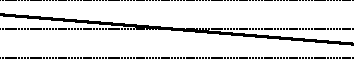
\includegraphics{images/contours-statement.pdf}%
	} //
	\gla Ang @ gihayo {} @ Pintemis minganeri-hen yona.//
	\glb ang= giha-yo Ø= Pintemis mingan-eri=hen yona //
	\glc \AgtT{}= blow-\TsgN{} \Top{}= {North Wind} ability-\Ins{}=all
		\TsgN{}.\Gen{}. //
	\glft `The North Wind blew with all of his might.' //
\endgl\xe

\subsubsection{Yes–no questions}
\index{questions|(}

Since Ayeri does not use a particle or word order to mark closed questions as 
such, intonation is used to mark the difference from a declarative statement. 
To achieve a strong contrast, questions exhibit gradually rising intonation:

\ex[belowexskip=0em]\begingl
	\glpreamble\adjustbox{valign=t}{%
		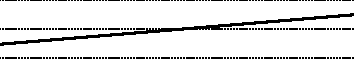
\includegraphics{images/contours-ynquestion.pdf}%
	} //
	\gla Ang @ gihayo {} @ Pintemis minganeri-hen yona? //
	\glb ang= giha-yo Ø= Pintemis mingan-eri=hen yona //
	\glc \AgtT{}= blow-\TsgN{} \Top{}= {North Wind} ability-\Ins{}=all
		\TsgN{}.\Gen{}. //
	\glft `Did the North Wind blow with all of his might?' //
\endgl\xe

\subsubsection{`Wh-' questions}

Unlike English\index{English}, Ayeri marks open questions with an in-situ question word.
Open questions are thus marked by the question word causing a sharp rise and 
fall in the overall contour of the question. The first half of the clause has 
the rising contour of a question, the second half has gradually falling pitch.

\ex[belowexskip=0em]\begingl
	\glpreamble\adjustbox{valign=t}{%
		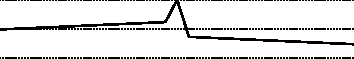
\includegraphics{images/contours-whquestion.pdf}%
	} //
	\gla Ang @ engyo mico sinya luga toya sam? //
	\glb ang= eng-yo mico sinya-Ø luga toya sam //
	\glc \AgtT{}= be.more-\TsgN{} strong who-\Top{} among \TplN{}.\Loc{}
		two //
	\glft `Who was the stronger of the two?' //
\endgl\xe

\index{questions|)}

\subsubsection{Lists}

List statements have the general gradual downward slope of declarative
statements, but the individual items can nonetheless be marked by a pitch rise
on the primary accent of each item.

\ex[belowexskip=0em]\begingl
	\glpreamble\adjustbox{valign=t}{%
		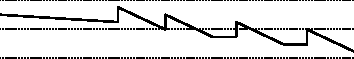
\includegraphics{images/contours-list.pdf}%
	} //
	\gla Le @ vacyeng seygo, disu, betay nay vasra. //
	\glb le= vac=yeng seygo-Ø disu-Ø betay-Ø nay vasra-Ø //
	\glc \PatTI{}= like=\TsgF{}.\Aarg{} apple-\Top{} banana-Ø berry-Ø and
		nut-Ø //
	\glft `She likes apples, bananas, berries and nuts.' //
\endgl\xe

\subsubsection{Complement and relative clauses}
\index{complement clause|(}
\index{relative clause|(}

Complement clauses\index{complement clause} are characterized by the short
spike at the end of the preceding main clause followed by a short break.
Together, these auditory clues signal the beginning of a new syntactic unit
within the context of the current sentence. This is broadly similar to list
statements. Otherwise, statements with complement clauses as well bear the
overall downward-sloping contour of declarative statements if included in such.

\ex\begingl
	\glpreamble\adjustbox{valign=t}{%
		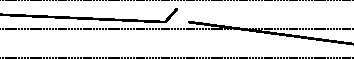
\includegraphics{images/contours-complement.pdf}%
	} //
	\gla Ang @ manga @ rantong, engyo mico sinyāng. //
	\glb ang= manga= ran=tong eng-yo mico sinya-ang //
	\glc \AgtT{}= \Prog{}= argue=\TplN{}.\Aarg{} be.more-\TsgN{} strong
		who-\Aarg{}//
	\glft `They were arguing who is stronger.' //
\endgl\xe

Relative clauses,\index{relative clause} on the other hand, do not receive 
special prosodic marking, but are treated the same as other basic sentence 
types. They display a continuous downward slope if part of a 
declarative statement, or a continuous upward slope if part of a question:

\pex[belowexskip=0em]
\a\begingl
	\glpreamble\adjustbox{valign=t}{%
		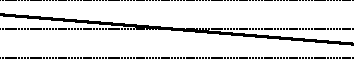
\includegraphics{images/contours-statement.pdf}%
	} //
	\gla Lugaya asāyāng si sitang-naykonyāng kong tovaya. //
	\glb luga-ya asāya-ang si sitang=naykon=yāng kong tova-ya mato //
	\glc pass-\TsgM{} traveler-\Aarg{} \Rel{} self=wrap=\TsgM{}.\Aarg{} 
		inside cloak-\Loc{} //
	\glft `A traveler passed who had wrapped himself into a cloak.' //
\endgl
\\

\a\label{ex:travelercoat}\begingl
	\glpreamble\adjustbox{valign=t}{%
		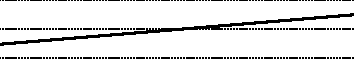
\includegraphics{images/contours-ynquestion.pdf}%
	} //
	\gla Adareng asāyās si le @ ninyāng tova? //
	\glb ada-reng asāya-as si le= nin=yāng tova-Ø //
	\glc that-\AargI{} traveler-\Parg{} \Rel{} \PatTI{}= wear=\TsgM{}.\Aarg{} 
		coat-\Top{} //
	\glft `Is that the traveler who wore the coat?' //
\endgl
\xe

\index{relative clause|)}
\index{complement clause|)}

\subsubsection{Contrast}

Ayeri uses a kind of topic system for highlighting constituents in a clause by
morphosyntactic means, but this is still different from emphasis on semantic
grounds, for example when the speaker wants to highlight a semantic difference
in the same syntactic position (compare focus, \autoref{subsec:focus}), as in
the following example, which presents a possible answer to the question posed in
(\ref{ex:travelercoat}):

\ex\begingl
	\glpreamble\adjustbox{valign=t}{%
		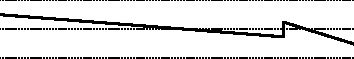
\includegraphics{images/contours-contrast.pdf}%
	} //
	\gla Adareng asāyās si le @ nin-yāng \upshape{kegan}. //
	\glb ada-reng asāya-as si le= nin=yāng kegan-Ø //
	\glc that-\AargI{} traveler-\Parg{} \Rel{} \PatTI{}= wear=\TsgM{}.\Aarg{} 
		hat-\Top{} //
	\glft `It is the traveler who wore the \emph{hat}.' //
\endgl\xe

We can see here a spike towards the end of the utterance where the word 
\xayr{kegnF}{kegan}{hat} is placed. This word receives extra stress for 
contrast with \xayr{tov}{tova}{coat}, which is what the other person had asked 
about.

\index{intonation|)}
